% PLEASE USE THIS FILE AS A TEMPLATE FOR THE PUBLICATION 
% Check file IOS-Book-Article.tex
%
\documentclass{IOS-Book-Article}
     %[seceqn,secfloat,secthm]
%\usepackage{mathptmx}
%\usepackage[T1]{fontenc}
%\usepackage{times}%
\usepackage{graphicx}
\usepackage{amsmath}
\usepackage{comment}
\newcommand{\ci}{\mathcal{I}}
\usepackage{paralist}
%
%%%%%%%%%%% Put your definitions here
%IMPORTANT: ONLY INCLUDE AS %IMPORTANT: ONLY INCLUDE AS %IMPORTANT: ONLY INCLUDE AS \input{idp-latex/idp-latex}
\usepackage{import}

\subimport{idp-latex/}{includes-no-theorems}
\subimport{idp-latex/}{common-citations}
\subimport{idp-latex/}{theorems}







%The following are directives for LaTeX editors that collect ``included files'' to autocomplete macros etcetera
\ignore{
\include{includes-no-theorems}
\include{common-citations}
\include{theorems}
}
\usepackage{import}

\subimport{idp-latex/}{includes-no-theorems}
\subimport{idp-latex/}{common-citations}
\subimport{idp-latex/}{theorems}







%The following are directives for LaTeX editors that collect ``included files'' to autocomplete macros etcetera
\ignore{
\usepackage{ifthen}
\usepackage{url}
% \usepackage{cite} DOES NOT WORK WITH ALL STYLES
\usepackage{amssymb}
\usepackage{amsmath}
\usepackage{import}
\subimport{packages/}{xparse}
\usepackage{amsmath}
\usepackage[usenames,dvipsnames]{xcolor}
\usepackage{xspace}
\usepackage{datatool}
\usepackage{glossaries}

%ensured math mode with correct spacing
\providecommand\m[1]{\ensuremath{#1}\xspace}
\renewcommand{\m}[1]{\ensuremath{#1}\xspace}
\newcommand{\trval}[1]{\m{\mathbf{#1}}}



%%%%%%%%%%%%%%%%%%%%%%%%%%%%%%%%%%%%%%%%%%%%%%%%%%%%%%%%%%%%%%%%%%%%%%%%%%%%
%%%%%%%%%         LOGICAL STUFF: Operators, theories, ....         %%%%%%%%%
%%%%%%%%%%%%%%%%%%%%%%%%%%%%%%%%%%%%%%%%%%%%%%%%%%%%%%%%%%%%%%%%%%%%%%%%%%%%

%NOTE: arrows are not surrounded by the \m command. THe reason is that they are math operators that have
% other spacing 
% For instance: L\to L has spacing between L and \to and betwee \to and L, while L{\to}L does not. 

%% Logic
% lor, land, lnot are standard. Extensions:
	\newcommand{\limplies}{\Rightarrow}
	\newcommand{\limpl}{\limplies}
	\newcommand{\lequiv}{\Leftrightarrow}
	\newcommand{\limpliedby}{\Leftarrow}
	\newcommand{\limplied}{\limpliedby}
	\newcommand{\lrule}{\leftarrow}
	\newcommand{\cause}{\stackrel{c}{\lrule}}
	\newcommand{\rul}{\leftarrow}
	\newcommand{\ltrue}{\trval{t}}
	\newcommand{\lfalse}{\trval{f}}
	\newcommand{\lunkn}{\trval{u}}
	\newcommand{\lincon}{\trval{i}}
%related
	\newcommand{\bigand}{\bigwedge}
	\newcommand{\bigor}{\bigvee}
	\newcommand{\true}{\m{\top}}
	\newcommand{\false}{\m{\bot}}
% Marc zijn versies
	\newcommand{\Lra}{\Leftrightarrow}
	\newcommand{\lra}{\leftrightarrow}
	\newcommand{\Ra}{\Rightarrow}
	\newcommand{\La}{\Leftarrow}
	\newcommand{\ra}{\rightarrow}
	\newcommand{\la}{\leftarrow}
	\newcommand{\mim}{\limplies}
	\newcommand{\equi}{\lequiv}
	\newcommand{\Tr}{\ltrue}
	\newcommand{\Fa}{\lfalse}
	\newcommand{\Un}{\lunkn}
	\newcommand{\In}{\lincon}
	
%Vocabularies, structures, theories
	\newcommand{\voc}{\m{\Sigma}}
	\newcommand{\invoc}{\m{\sigma_{in}}}
	\newcommand{\outvoc}{\m{\sigma_{out}}}
	\newcommand{\struct}{\m{I}}
	\newcommand{\structx}{\m{I}}
	\newcommand{\I}{\m{\mathcal{I}}}
	\newcommand{\Iin}{\m{\I_{in}}}
	\newcommand{\J}{\m{\mathcal{J}}}
	\newcommand{\instruct}{\m{I_{in}}}
	\newcommand{\outstruct}{\m{I_{out}}}
	\newcommand{\theory}{\m{\mathcal{T}}}

%More caligraphic characters
	\newcommand{\PP}{\m{\mathcal{P}}}
	\newcommand{\LL}{\m{\mathcal{L}}}
	\newcommand{\WW}{\m{\mathcal{W}}}
	\newcommand{\BB}{\m{\mathcal{B}}}


%Often used abbreviations for definitions, formulas,...
	\newcommand{\D}{\m{\Delta}}
	\newcommand{\f}{\m{\varphi}}
	\newcommand{\atom}{\m{a}}
	\newcommand{\lit}{\m{l}}
	\newcommand{\rules}{\m{R}}
	\newcommand{\set}{\m{S}}
	\NewDocumentCommand\inter{g+g}{%
	  \IfNoValueTF{#1}
	    {\struct}
	    {\m{#1^{#2}}}}
	\newcommand{\partinter}{\m{J}}
	\newcommand{\model}{\m{M}}
	\newcommand{\fone}{\m{\varphi}}
	\newcommand{\ftwo}{\m{\psi}}

%properties of definitions
	\newcommand{\defined}[1]{\ensuremath{\mbox{\it Def}({#1})}\xspace}
	\newcommand{\open}[1]{\ensuremath{\mbox{\it Open}({#1})}\xspace}
	\newcommand{\pars}[1]{\ensuremath{\mbox{\it Par}({#1})}\xspace}
	\newcommand{\just}{\m{just}}

% Inferences
	\newcommand{\mx}[3]{\m{<#1, #2, #3>}}

%Vectors
	\newcommand{\xxx}{\m{\overline{x}}}
	\newcommand{\XXX}{\m{\overline{X}}}
	\newcommand{\yyy}{\m{\overline{y}}}
	\newcommand{\zzz}{\m{\overline{z}}}
	\newcommand{\ddd}{\m{\overline{d}}}
	\newcommand{\eee}{\m{\overline{e}}}
	\newcommand{\ccc}{\m{\overline{c}}}
	\newcommand{\bracketddd}{\m{\big(\overline{d}\big)}}
	\newcommand{\bddd}{\m{\big(\overline{d}\big)}}
	\newcommand{\DDD}{\m{\overline{D}}}
	\newcommand{\vvv}{\m{\overline{v}}}
	\newcommand{\ttt}{\m{\overline{t}}}
	\newcommand{\aaa}{\m{\overline{a}}}
	\newcommand{\bbb}{\m{\overline{b}}}
 	\providecommand{\lll}{\m{\overline{l}}}%sometimes, already exists
 	\renewcommand{\lll}{\m{\overline{l}}}
	\newcommand{\TTT}{\m{\overline{T}}}

%Set operations
	\newcommand{\elim}{\m{\backslash}}
	
%Rewrite rules
	\newcommand{\transformarrow}{\pmb{\pmb\rightarrowtail}}
	\newcommand{\rewrite}[2]{\m{#1  \ \transformarrow\    #2 }}

% Common Base types
	\newcommand{\bool}{\m{\mathbb{B}}}
	\newcommand{\Bool}{\bool}
	\newcommand{\nat}{\m{\mathbb{N}}}
	\newcommand{\Nat}{\nat}
	\renewcommand{\int}{\m{\mathbb{Z}}}
	\newcommand{\real}{\m{\mathbb{R}}}
	\newcommand{\rat}{\m{\mathbb{Q}}}

% Precision order
	\newcommand{\leqp}{\m{\leq_p}}
	\newcommand{\geqp}{\m{\geq_p}}
	\newcommand{\leqk}{\m{\leq_k}}
	\newcommand{\geqk}{\m{\geq_k}}
	\newcommand{\leqt}{\m{\leq_t}}
	\newcommand{\geqt}{\m{\geq_t}}
	
%Lattice operators
	\DeclareMathOperator\glb{glb}
	\DeclareMathOperator\lub{lub}
	\DeclareMathOperator\lfp{lfp}
	\DeclareMathOperator\gfp{gfp}


%valuations
	\newcommand{\val}{\m{\nu}}
	\newcommand{\superval}{\m{sv}}
	\newcommand{\kleeneval}{\m{Kl}}



%other
	\newcommand{\typed}[2]{\m{#1\in #2:}}
	\newcommand{\hasmodel}{\mid\!\equiv}
	\NewDocumentCommand\subs{g+g}{%
	  \IfNoValueTF{#1}
	    {\m{/}}
	    {\m{#1/ #2}}}
	\newcommand{\substitute}[2]{\subs{#1}{#2}}	
	\newcommand{\func}[1]{\m{f(#1)}}
	\newcommand{\setof}[1]{\m{\left \{ #1 \right \}}}
	\newcommand{\tuple}[1]{\m{\left \langle #1 \right \rangle }}
	\newcommand{\til}{\m{\sim}}
	\newcommand\eqdef{\mathrel{\overset{\makebox[0pt]{\mbox{\normalfont\tiny\sffamily def}}}{=}}}



%%%%%%%%%%%%%%%%%%%%%%%%%%%%%%%%%%%%%%%%%%%%%%%%%%%%%%%%%%%%%%%%%%%%%%%%%%%%
%%%%%%%%%                    Logics and systems                    %%%%%%%%%
%%%%%%%%%%%%%%%%%%%%%%%%%%%%%%%%%%%%%%%%%%%%%%%%%%%%%%%%%%%%%%%%%%%%%%%%%%%%

%General command to ensure correct spacing and text mode
	\newcommand{\logicname}[1]{\textsc{#1}\xspace}

%Systems
	\newcommand{\idp}{\logicname{IDP}}
	\newcommand{\xsb}{\logicname{XSB}}
	\newcommand{\idptwo}{\logicname{IDP$^2$}}
	\newcommand{\idpthree}{\logicname{IDP3}}
	\newcommand{\idpfour}{\logicname{IDP4}}
	\newcommand{\idpdraw}{\logicname{ID$^{P}_{Draw}$}}
	\newcommand{\idpide}{\logicname{ID$^{P}_{E}$}}
	\newcommand{\minisat}{\logicname{MiniSAT}}
	\newcommand{\minisatid}{\logicname{MiniSAT(ID)}}
	\newcommand{\gidl}{\logicname{GidL}}
	\newcommand{\sts}{\logicname{SAT-to-SAT}}
	\newcommand{\breakid}{\logicname{BreakID}}
	\newcommand{\glucose}{\logicname{Glucose}}
	\newcommand{\shatter}{\logicname{Shatter}}
	\newcommand{\saucy}{\logicname{Saucy}}
	\newcommand{\sbass}{\logicname{sbass}}
	\newcommand{\nauty}{\logicname{nauty}}
	\newcommand{\bliss}{\logicname{bliss}}
	\newcommand{\gringo}{\logicname{gringo}}
	\newcommand{\lparse}{\logicname{Lparse}}
	\newcommand{\smodels}{\logicname{Smodels}}
	

	
%logics
	\newcommand{\fodotidp}{\logicname{FO(\ensuremath{\cdot})\ensuremath{^{\mathtt{IDP}}}}}
	\newcommand{\foidp}{\fodotidp}
	\newcommand{\fodot}{\logicname{FO(\ensuremath{\cdot})}}
	\newcommand{\pcdot}{\logicname{PC(\ensuremath{\cdot})}}
	\newcommand{\foid}{\logicname{FO(ID)}}
	\newcommand{\foidaggpf}{\logicname{FO(ID,\allowbreak Agg,\allowbreak PF)}}
	\newcommand{\foidaggpft}{\logicname{FO(ID,\allowbreak Agg,\allowbreak PF,\allowbreak T)}}
	\newcommand{\foidplus}{\logicname{C-Log}} %DEPRECATED
	\newcommand{\clog}{\logicname{C-Log}}
	\newcommand{\foclog}{\logicname{FO(C)}}
	\newcommand{\hoid}{\logicname{HO(ID)}}
	\newcommand{\hopfid}{\logicname{HO(PF,ID)}}
	\newcommand{\fo}{\FO}
	\newcommand{\esoid}{\logicname{\ensuremath{\exists}SO(ID)}}
	\newcommand{\cpl}{\logicname{CP}-logic\xspace}
	\newcommand{\aspcore}{\text{\sc ASP-Core-2}\xspace}

%acronyms. USAGE: \ouracronym{CommandName}{A}{Acronym} creates a command \CommandName such that:
% * The first time you write it (probably the moment you define it), it reads Acronym (A)
% * All later times you use it, it simply says A.
% NOTE: to reset the counter, use \glsreset{<label>}
\newcommand{\ouracronym}[3]{%
	\newacronym{#1}{#2}{#3}
	\expandafter\newcommand\csname #1\endcsname{\gls{#1}\xspace}%
}
	\ouracronym{FO}{FO}{first-order logic}
	\ouracronym{PC}{PC}{propositional calculus}
	\ouracronym{MX}{MX}{Model Expansion}
	\ouracronym{MO}{MO}{Model Optimization}
	\ouracronym{ASP}{ASP}{Answer Set Programming}
	\ouracronym{TP}{TP}{Theorem Proving}
	\ouracronym{LP}{LP}{Logic Programming}
	\ouracronym{CP}{CP}{Constraint Programming}
	\ouracronym{FP}{FP}{Functional Programming}
	\ouracronym{KR}{KR}{Knowledge Representation}
	\ouracronym{CSP}{CSP}{Constraint Satisfaction Problem}
	\ouracronym{SMT}{SMT}{SAT Modulo Theories}
	\ouracronym{KBS}{KBS}{knowledge base system}
	\ouracronym{NNF}{NNF}{Negation Normal Form}
	\ouracronym{FNNF}{FNNF}{Flat Negation Normal Form}
	\ouracronym{DefNNF}{DefNNF}{Definition Negation Normal Form}
	\ouracronym{DEFNF}{DEFNF}{Definition Normal Form}
	\newcommand{\DEFNNF}{\DefNNF} %Was previously called like this. Keeping consistency
	\ouracronym{CDCL}{CDCL}{Conflict-Driven Clause-Learning}
	\ouracronym{WFS}{WFS}{Well-Founded Semantics}
	\ouracronym{LCG}{LCG}{Lazy Clause Generation}
	\ouracronym{AEL}{AEL}{Autoepistemic Logic}
	\ouracronym{OEL}{OEL}{Ordered Epistemic Logic}
	\ouracronym{AFT}{AFT}{Approximation Fixpoint Theory}

%%%%%%%%%%%%%%%%%%%%%%%%%%%%%%%%%%%%%%%%%%%%%%%%%%%%%%%%%%%%%%%%%%%%%%%%%%%%
%%%%%%%%%       DEFINITIONS: commands for writing definitions      %%%%%%%%%
%%%%%%%%%%%%%%%%%%%%%%%%%%%%%%%%%%%%%%%%%%%%%%%%%%%%%%%%%%%%%%%%%%%%%%%%%%%%

%%%%%%%%%%%%%%%%%%%%%%%%%%%%%%%%%%%%%
%   Stuff for (delayed) definitions   %
%%%%%%%%%%%%%%%%%%%%%%%%%%%%%%%%%%%%%

% The only commands you should use explicitly are:
%	* Environment ldef for a logical definition (should be used in mathmode)
%	* Environment ltheo for a logical theory (starts mathmode itself)
%	* \LRule defines a rule, usage \LRule{HEAD}{BODY}{OPTIONAL: DELAY}{OPTIONAL: CONSTRUCTION}
% 		---> Can be used inside a ldef or an align environment
%% USAGE EXAMPLE:
% \begin{ltheo}
% \lnot S(1) \\
% \exists x\typed{D}: P(x) \\
% \forall x\typed{D}: P(x) \limpl R(x)\\
% \begin{ldef}
% \LRule{\forall x\typed{D}: R(x)}{ Q(x) \lor S(x)}{delay}{construction} \\
% \LRule{\forall x\typed{D}: R(x)}{ Q(x) \lor S(x)}{delay}{construction} \\
% \LRule{\forall x\typed{D}: R(x)}{ Q(x) \lor S(x)}{delay}{construction} \\
% \LRule{\forall x\typed{D}: Q(x)}{ R(x)}
% \end{ldef}
% \end{ltheo}
%
% You can use these rules in an align environment as follows:
% \begin{align*}
% \LRule{\forall x\typed{D}: R(x)}{ Q(x) \lor S(x)}{delay}{construction} \\
% \LRule{\forall x\typed{D}: R(x)}{ Q(x) \lor S(x)}{delay}{construction} \\
% \LRule{Q}{ R(x)}
% \end{align*}

	\makeatletter
	\def\ifenv#1{
	\def\@tempa{#1}%
	\def\@ttempa{#1*}%
	\ifx\@tempa\@currenvir
	\expandafter\@firstoftwo
	\else
	\expandafter\@secondoftwo
	\fi
	}
	\makeatother

%Delayed definition rule. Usage: \ddrule{HEAD}{BODY}{DELAY}{CONSTRUCTION}
	\newcommand{\ddrule}[4]{\ensuremath{#1 \leftarrow #2 & \{#3\} & #4}}
%Non-delayed definition rule. Usage: \drule{HEAD}{BODY}
	\newcommand{\drule}[2]{\ensuremath{#1 & \leftarrow & #2}}

%Delayed align rule. Usage: \darule{HEAD}{BODY}{DELAY}{CONSTRUCTION}
	\newcommand{\darule}[4]{\ensuremath{#1 \leftarrow #2 & \{#3\} & #4}}
%Non-delayed align rule. Usage: \arule{HEAD}{BODY}
	\newcommand{\arule}[2]{\ensuremath{#1 \, &\leftarrow \, #2}}

	\newenvironment{ldef}{\left\{\begin{array}{l@{ \,}l@{\,}l}}{\end{array}\right\}}
	\newenvironment{ltheo}{\[\begin{array}{l}}{\end{array}\]\ignorespacesafterend}

	\newcommand{\LNDRule}[2]{
	\ifenv{array}
	{\drule{#1}{#2}}
	{ \ifenv{align}
		{\arule{#1}{#2}}
		{\ifenv{align*}
		{\arule{#1}{#2}}
		{ERROR: using LDRule in unsupported environment: \@currenvir}
		}
	}
	}

	\newcommand{\LDRule}[4]{
	\ifenv{array}
	{\ddrule{#1}{#2}{#3}{#4}}
	{ \ifenv{align}
		{\darule{#1}{#2}{#3}{#4}}
		{\ifenv{align*}
		{\darule{#1}{#2}{#3}{#4}}
		{ERROR: using LDRule in unsupported environment: \@currenvir}
		}
	}
	}

% NOTE: if getting strange errors on alignments, you probably forgot the ldef environment
	\NewDocumentCommand\LRule{m+g+g+g}{%
		\IfNoValueTF{#2}%
		{#1.&}{%
		\IfNoValueTF{#3}
		{\LNDRule{#1}{#2.}}
		{\LDRule{#1}{#2.}{#3}{#4}}%
		}
	}



%FOR COMPLEX RULES: with a c above the lrule...

	\NewDocumentCommand\CLRule{m+g}{%
	\ifenv{array}
	{\cdrule{#1}{#2}}
	{ \ifenv{align}
		{\carule{#1}{#2}}
		{\ifenv{align*}
			{\carule{#1}{#2}}
			{ERROR: using CLRule in unsupported environment: \@currenvir}
		}
	}
	}

	\NewDocumentCommand\carule{m+g}{%
		\IfNoValueTF{#2}
			{\ensuremath{#1.}}
			{\ensuremath{#1 \, &\cause \, #2}}}
	\NewDocumentCommand\cdrule{m+g}{%
		\IfNoValueTF{#2}
			{\ensuremath{#1.}}
			{\ensuremath{#1 & \cause & #2}}}
	



%%%%%%%%%%%%%%%%%%%%%%%%%%%%%%%%%%%%%%%%%%%%%%%%%%%%%%%%%%%%%%%%%%%%%%%%%%%%
%            Stuff for rules for state-changes in an algorithm             %
%%%%%%%%%%%%%%%%%%%%%%%%%%%%%%%%%%%%%%%%%%%%%%%%%%%%%%%%%%%%%%%%%%%%%%%%%%%%

% The only commands you should use explicitly are:
%	* Environment lprop for a set of state-changing rules
%	* \AlgoRule defines a propagation rule, usage \AlgoRule{Name}{Previous state}{New state}{Condition}
% The whole environment is in MATH mode by default, so use hbox to obtain normal text.

	\newcommand{\algrule}[4]{
	\hbox{{#1}:}& 
	\quad #2 ~\longrightarrow~ #3 
	\hbox{~ if } #4\\
	}

	\newenvironment{lprop}{\[\begin{array}{ll}}{\end{array}\]}

	\newcommand{\AlgoRule}[4]{
	\ifenv{array}
	{\algrule{#1}{#2}{#3}{#4}}
		{ERROR: using AlgoRule in unsupported environment: \@currenvir}
	}


\newcommand{\commentstyle}{\color{Gray}}



%%%%%%%%%%%%%%%%%%%%%%%%%%%%%%%%%%%%%%%%%%%%%%%%%%%%%%%%%%%%%%%%%%%%%%%%%%%%
%%%%%%%                    In-paper commentstyle                     %%%%%%%
%%%%%%%%%%%%%%%%%%%%%%%%%%%%%%%%%%%%%%%%%%%%%%%%%%%%%%%%%%%%%%%%%%%%%%%%%%%%

	\newcommand{\ignore}[1]{}

%Boolean to quickly disable all comments
	\newboolean{nocomments}
	\setboolean{nocomments}{false}

%Boolean to decide whether we put our name in margin or not
	\newboolean{commentmargin}
	\setboolean{commentmargin}{true}

%General comments
	\newcommand{\namedcomment}[3]{%
		\ifthenelse{\boolean{nocomments}}%
		{}%IF no comments, write nothing
		{%Otherwise
			\ifthenelse{\boolean{commentmargin}}%
				{ {\color{#3} \marginpar{\color{#3}\sc #2}#1}  }%Name in margin
				{  {\color{#3} {\sc #2}: #1}  }%Name not in margin
		}%
	}
	\newcommand{\mnamedcomment}[3]{\ifthenelse{\boolean{nocomments}}{}{{\marginpar{ \color{#3}{\sc #2}:#1}}}}

	\newcommand{\namedchange}[4]{\marginpar{\color{#4}\sc #3}\textcolor{#4}{#1}\textcolor{gray}{\st{#2}}}

%todo's
	\newcommand{\todo}[1]{\namedcomment{#1}{TODO}{blue}}
	\newcommand{\todonm}[1]{{\color{blue}\sc TODO} #1}
	\newcommand{\mtodo}[1]{\mnamedcomment{#1}{TODO}{blue}}
	\newcommand{\old}[1]{\namedcomment{#1}{OLD}{gray}}

%Personal comments (KRR):
	\newcommand{\bart}[1]{\namedcomment{#1}{bb}{red}}
	\newcommand{\mbart}[1]{\mnamedcomment{#1}{bb}{red}}
	\newcommand{\gerda}[1]{\namedcomment{#1}{gj}{orange}}
	\newcommand{\marc}[1]{\namedcomment{#1}{md}{orange}}
	\newcommand{\joost}[1]{\namedcomment{#1}{jv}{purple}}
	\newcommand{\bdc}[1]{\namedcomment{#1}{bdc}{OliveGreen}}
	\newcommand{\broes}[1]{\namedcomment{#1}{bdc}{OliveGreen}}
	\newcommand{\mbroes}[1]{\mnamedcomment{#1}{bdc}{OliveGreen}}
	\newcommand{\pieter}[1]{\namedcomment{#1}{pvh}{NavyBlue}}
	\newcommand{\maurice}[1]{\namedcomment{#1}{mb}{orange}}
	\newcommand{\ingmar}[1]{\namedcomment{#1}{id}{purple}}
	\newcommand{\matthias}[1]{\namedcomment{#1}{mvdh}{blue}}
	\newcommand{\mmaurice}[1]{\mnamedcomment{#1}{mb}{orange}}
	\newcommand{\jo}[1]{ \namedcomment{#1}{jo}{Fuchsia}}
	\newcommand{\joachim}[1]{ \namedcomment{#1}{jj}{Sepia}}
	\newcommand{\mjoachim}[1]{ \mnamedcomment{#1}{jj}{Sepia}}
	\newcommand{\tim}[2]{\namedcomment{#1}{tvde}{brown}}
	\usepackage{soul}
	\newcommand{\bartch}[2]{\namedchange{#1}{#2}{bb}{red}}
	\newcommand{\broesch}[2]{\namedchange{#1}{#2}{bdc}{OliveGreen}}
%Personal comments  (Collaborations):
	\newcommand{\pjs}[1]{\namedcomment{#1}{pjs}{orange}}
	\newcommand{\jan}[1]{\namedcomment{#1}{jvdb}{orange}}
	\newcommand{\jvt}[1]{\namedcomment{#1}{jvt}{orange}}
	\newcommand{\aw}[1]{\namedcomment{#1}{aw}{orange}}


%%%%%%%%%%%%%%%%%%%%%%%%%%%%%%%%%%%%%%%%%%%%%%%%%%%%%%%%%%%%%%%%%%%%%%%%%%%%
%%%%%%%                   Useful in-text commands                    %%%%%%%
%%%%%%%%%%%%%%%%%%%%%%%%%%%%%%%%%%%%%%%%%%%%%%%%%%%%%%%%%%%%%%%%%%%%%%%%%%%%

% \newcommand{\keyword}[2]{%
% 	\expandafter\newcommand\csname #1\endcsname{#2\xspace}%
% 	\expandafter\newcommand\csname #1s\endcsname{#2s\xspace}%
% 	\expandafter\newcommand\csname #1ness\endcsname{#2ness\xspace}%
% % 	\expandafter\newcommand\MakeUppercase{\csname #1\endcsname}{#2\xspace}%
% %	\expandafter\newcommand\csname\makefirstuc{#1}\endcsname{\makefirstuc{#2}\xspace}%
% %	\expandafter\newcommand\csname\makefirstuc{#1}\endcsname{\makefirstuc{#2}s\xspace}%
% }

\newcommand{\superscript}[1]{\ensuremath{^{\textrm{#1}}}}
\newcommand{\subscript}[1]{\ensuremath{_{\textrm{#1}}}}
\usepackage{etoolbox}

\newcommand\setcitation[2]{%
  \csdef{mycommoncitation#1}{#2}}
\newcommand\getcitation[1]{%
  \csuse{mycommoncitation#1}}

\setcitation{IDP}{WarrenBook/DeCatBBD14}
\setcitation{idp}{WarrenBook/DeCatBBD14}
\setcitation{fodot}{tocl/DeneckerT08}
\setcitation{foid}{tocl/DeneckerT08}
\setcitation{cplogic}{journal/tplp/VennekensDB10}
\setcitation{CPlogic}{journal/tplp/VennekensDB10}
\setcitation{CP}{Apt03}
\setcitation{cp}{Apt03}
\setcitation{EZCSP}{lpnmr/Balduccini11}
\setcitation{KR}{Baral:2003}
\setcitation{ASPComp2}{lpnmr/DeneckerVBGT09}
\setcitation{ASPComp3}{journals/tplp/CalimeriIR14}
\setcitation{ASPComp4}{conf/lpnmr/AlvianoCCDDIKKOPPRRSSSWX13}
\setcitation{ASPComp6}{jair/GebserMR17}
\setcitation{CPSupport}{ictai/DeCat13}
\setcitation{CPsupport}{ictai/DeCat13}
\setcitation{functionDetection}{iclp/DeCatB13}
\setcitation{fodot2asp}{DeneckerLTV12} %TODO replace by journal publication if one is publishedr
\setcitation{Tarskian}{DeneckerLTV12} %Same as the one above 
\setcitation{Inca}{iclp/DrescherW12}
\setcitation{csp2asp}{ijcai/DrescherW11}
\setcitation{DPLLT}{cav/GanzingerHNOT04}
\setcitation{AspInPractice}{synthesis/2012Gebser}
\setcitation{clasp}{ai/GebserKS12}
\setcitation{oclingo}{kr/GebserGKOSS12}
\setcitation{gringo}{lpnmr/GebserST07}
\setcitation{cmodels}{aaai/GiunchigliaLM04}
\setcitation{inputster}{tplp/Jansen13}
\setcitation{DLV}{tocl/LeonePFEGPS06}
\setcitation{LearningPaper}{TPLP/BruynoogheBBDDJLRDV} %TODO replace by published version
\setcitation{clog}{iclp/BogaertsVDV14} %TODO replace by journal publication if one is published
\setcitation{foc}{iclp/BogaertsVDV14}
\setcitation{FOC}{iclp/BogaertsVDV14}
\setcitation{inferenceClog}{ecai/BogaertsVDV14}
\setcitation{examplesClog}{nmr/BogaertsVDV14b} %TODO replace by better publication if possible
\setcitation{AFT}{DeneckerBV12}
\setcitation{KBS}{iclp/DeneckerV08}
\setcitation{KBS-invitedtalk}{jelia/Denecker16}
\setcitation{KBPE}{inap/DePooterWD11}
\setcitation{lazyGrounding}{jair/CatDBS15} 
\setcitation{LazyGrounding}{jair/CatDBS15} 
\setcitation{lazygrounding}{jair/CatDBS15} 
\setcitation{lazygroundingASP}{ijcai/BogaertsW18} 
\setcitation{ASP}{marek99stable}
\setcitation{satid}{sat/MarienWDB08}
\setcitation{lazyclausegeneration}{constraints/OhrimenkoSC09}
\setcitation{FP}{ACMCS/Hudak89}
\setcitation{GroundingWithBounds}{jair/WittocxMD10}
\setcitation{SAT}{faia/SilvaLM09}
\setcitation{LTC}{iclp/Bogaerts14}
\setcitation{SPSAT}{ictai/DevriendtBMDD12}
\setcitation{BreakID}{sat/DevriendtBBD16}
\setcitation{breakid}{sat/DevriendtBBD16}
\setcitation{LCG}{stuckeyLCG}
\setcitation{MiniZinc}{conf/cp/NethercoteSBBDT07}
\setcitation{minizinc}{conf/cp/NethercoteSBBDT07}
\setcitation{amadini}{cpaior/AmadiniGM13}
\setcitation{bootstrapping}{ngc/BogaertsJDJBD16}
\setcitation{Bootstrapping}{ngc/BogaertsJDJBD16}
\setcitation{GroundedFixpoints}{ai/BogaertsVD15}
\setcitation{PartialGroundedFixpoints}{ijcai/BogaertsVD15}
\setcitation{LogicBlox}{datalog/GreenAK12}
\setcitation{proB}{journals/sttt/LeuschelB08}
\setcitation{NaturalInductions}{KR/DeneckerV14} %TODO replace by journal publication if one is published
\setcitation{LP}{jacm/EmdenK76}
\setcitation{SMT}{faia/BarrettSST09}
\setcitation{AF}{ai/Dung95}
\setcitation{ADF}{kr/BrewkaW10}
\setcitation{af}{ai/Dung95}
\setcitation{adf}{kr/BrewkaW10}
\setcitation{ADFRevisited}{ijcai/BrewkaSEWW13}
\setcitation{adfrevisited}{ijcai/BrewkaSEWW13}
\setcitation{DefaultLogic}{ai/Reiter80}
\setcitation{DL}{ai/Reiter80}
\setcitation{AEL}{mo85}
\setcitation{minisat}{sat/EenS03}
\setcitation{completion}{adbt/Clark78}
\setcitation{wasp}{lpnmr/AlvianoDFLR13}
\setcitation{minisatid}{ictai/DeCat13}
\setcitation{lcg}{stuckeyLCG}
\setcitation{CEGAR}{jacm/ClarkeGJLV03}
\setcitation{cegar}{jacm/ClarkeGJLV03}
\setcitation{CuttingPlane}{or/DantzigFJ54}
\setcitation{kodkod}{tacas/TorlakJ07}
\setcitation{cdcl}{Marques-SilvaS99}
\setcitation{CDCL}{Marques-SilvaS99}
\setcitation{1UIP}{iccad/ZhangMMM01}
\setcitation{relevance}{ijcai/JansenBDJD16}
\setcitation{relevance-implementation}{aspocp/JansenBDJD16}
\setcitation{WFS}{GelderRS91}
\setcitation{wfs}{GelderRS91}
\setcitation{UnfoundedSet}{GelderRS91}
\setcitation{stablesemantics}{iclp/GelfondL88}
\setcitation{StableSemantics}{iclp/GelfondL88}
\setcitation{shatter}{Shatter}
\setcitation{sbass}{drtiwa11a}
\setcitation{lparsemanual}{url:lparse_manual}
\setcitation{AIC}{ppdp/FlescaGZ04}
\setcitation{templates}{tplp/DassevilleHJD15}
\setcitation{templates2}{iclp/DassevilleHBJD16}
\setcitation{sat-to-sat}{aaai/JanhunenTT16}
\setcitation{sat-to-sat-qbf}{bnp/BogaertsJT16}
\setcitation{sat-to-sat-QBF}{bnp/BogaertsJT16}
\setcitation{sat-to-sat-SO}{kr/BogaertsJT16}
\setcitation{XSB}{SwiW12}
\setcitation{KCmap}{jair/DarwicheM02}
\setcitation{TLA}{DBLP:books/aw/Lamport2002}
\setcitation{EventB}{BookAbrial2010}
\setcitation{MX}{MitchellTHM06}
\setcitation{MIP}{Sierksma96}
\setcitation{perefectmodel}{minker88/Przymusinski88}
\setcitation{SafeInductions}{ijcai/BogaertsVD17}
\setcitation{AIC}{ppdp/FlescaGZ04}
\setcitation{aic}{ppdp/FlescaGZ04}
\setcitation{alpha}{lpnmr/Weinzierl17}
\setcitation{omiga}{jelia/Dao-TranEFWW12}
\setcitation{gasp}{fuin/PaluDPR09}
\setcitation{asperix}{lpnmr/LefevreN09a}
\setcitation{CTL}{lop/ClarkeE81}
\setcitation{AFT-AIC}{ai/BogaertsC18}
\setcitation{UltimateApproximator}{DeneckerMT04}
\setcitation{KripkeKleene}{Fitting85}
\setcitation{AFT-HO}{corr/CharalambidisRS18} %TODO replace
\setcitation{HereThere}{Heyting30}
\setcitation{dAEL}{ijcai/HertumCBD16}
\setcitation{SDD}{ijcai/Darwiche11}
\setcitation{HEX}{ijcai/EiterIST05}
\setcitation{wADF}{aaai/BrewkaSWW18}
\setcitation{wADFfix}{corr/BrewkaSWW18}
\setcitation{}{}
\setcitation{}{}
\setcitation{}{}
\setcitation{}{}
\setcitation{}{}
\setcitation{}{}
\setcitation{}{}
\setcitation{}{}
\setcitation{}{}
\setcitation{}{}
\setcitation{}{}
\setcitation{}{}
\setcitation{}{}
  
 %Command for in case you want multiple citations in one, e.g., \cite{\refto{fodot},\refto{idp}}
 %Warning: no safety checks
\newcommand\refto[1]{%
      \getcitation{#1}}
      
 %usage: \mycite{key}, e.g., \mycite{fodot} results in \cite{tocl/DeneckerT08}
\newcommand\mycite[1]{%
      \ifcsname mycommoncitation#1\endcsname%
   \cite{\getcitation{#1}}%
  \else%
    \cite{#1}%
  \fi%
}	
  
   %usage: \mycite{key}, e.g., \mycite{fodot} results in \cite{tocl/DeneckerT08}
\newcommand\mycitet[1]{%
      \ifcsname mycommoncitation#1\endcsname%
   \citet{\getcitation{#1}}%
  \else%
    \citet{#1}
  \fi%
}	
  

\usepackage{amsthm}
\usepackage{thmtools}

\declaretheorem[style=plain,	name=Theorem,		numberwithin=section]{thm}
\declaretheorem[style=plain,	name=Theorem,		numberlike=thm]{theorem}
\declaretheorem[style=plain,	name=Proposition,	numberlike=thm]{prop}
\declaretheorem[style=plain,	name=Proposition,	numberlike=thm]{proposition}
\declaretheorem[style=plain,	name=Lemma,		numberlike=thm]{lem}
\declaretheorem[style=plain,	name=Lemma,		numberlike=thm]{lemma}
\declaretheorem[style=plain,	name=Lemma,		numbered=no]   {lem*}
\declaretheorem[style=plain,	name=Corollary,		numberlike=thm]{cor}
\declaretheorem[style=plain,	name=Corollary,		numberlike=thm]{corollary}
\declaretheorem[style=plain,	name=Conjecture,	numberlike=thm]{conjecture}

\declaretheorem[style=definition,	name=Definition,	numberlike=thm]{definition}
\declaretheorem[style=definition,	name=Definition,	numberlike=thm]{defn}
\declaretheorem[style=definition,	qed=$\blacktriangle$,	numberlike=thm]{example}
\declaretheorem[style=definition,	qed=$\blacktriangle$,	numberlike=thm]{ex}
\declaretheorem[style=definition,	qed=$\blacktriangle$,	numbered=no]{ex*}

\declaretheorem[style=remark,		name=Notation,		numberlike=thm]{nota}
\declaretheorem[style=remark,	name=Notation,		numbered=no]{nota*}
\declaretheorem[style=remark,	name=Note,		numberlike=thm]{note}
\declaretheorem[style=remark,	name=Note,		numbered=no]{note*}
\declaretheorem[style=remark,	name=Remark,		numberlike=thm]{remark}



}
\usepackage{import}

\subimport{idp-latex/}{includes-no-theorems}
\subimport{idp-latex/}{common-citations}
\subimport{idp-latex/}{theorems}







%The following are directives for LaTeX editors that collect ``included files'' to autocomplete macros etcetera
\ignore{
\usepackage{ifthen}
\usepackage{url}
% \usepackage{cite} DOES NOT WORK WITH ALL STYLES
\usepackage{amssymb}
\usepackage{amsmath}
\usepackage{import}
\subimport{packages/}{xparse}
\usepackage{amsmath}
\usepackage[usenames,dvipsnames]{xcolor}
\usepackage{xspace}
\usepackage{datatool}
\usepackage{glossaries}

%ensured math mode with correct spacing
\providecommand\m[1]{\ensuremath{#1}\xspace}
\renewcommand{\m}[1]{\ensuremath{#1}\xspace}
\newcommand{\trval}[1]{\m{\mathbf{#1}}}



%%%%%%%%%%%%%%%%%%%%%%%%%%%%%%%%%%%%%%%%%%%%%%%%%%%%%%%%%%%%%%%%%%%%%%%%%%%%
%%%%%%%%%         LOGICAL STUFF: Operators, theories, ....         %%%%%%%%%
%%%%%%%%%%%%%%%%%%%%%%%%%%%%%%%%%%%%%%%%%%%%%%%%%%%%%%%%%%%%%%%%%%%%%%%%%%%%

%NOTE: arrows are not surrounded by the \m command. THe reason is that they are math operators that have
% other spacing 
% For instance: L\to L has spacing between L and \to and betwee \to and L, while L{\to}L does not. 

%% Logic
% lor, land, lnot are standard. Extensions:
	\newcommand{\limplies}{\Rightarrow}
	\newcommand{\limpl}{\limplies}
	\newcommand{\lequiv}{\Leftrightarrow}
	\newcommand{\limpliedby}{\Leftarrow}
	\newcommand{\limplied}{\limpliedby}
	\newcommand{\lrule}{\leftarrow}
	\newcommand{\cause}{\stackrel{c}{\lrule}}
	\newcommand{\rul}{\leftarrow}
	\newcommand{\ltrue}{\trval{t}}
	\newcommand{\lfalse}{\trval{f}}
	\newcommand{\lunkn}{\trval{u}}
	\newcommand{\lincon}{\trval{i}}
%related
	\newcommand{\bigand}{\bigwedge}
	\newcommand{\bigor}{\bigvee}
	\newcommand{\true}{\m{\top}}
	\newcommand{\false}{\m{\bot}}
% Marc zijn versies
	\newcommand{\Lra}{\Leftrightarrow}
	\newcommand{\lra}{\leftrightarrow}
	\newcommand{\Ra}{\Rightarrow}
	\newcommand{\La}{\Leftarrow}
	\newcommand{\ra}{\rightarrow}
	\newcommand{\la}{\leftarrow}
	\newcommand{\mim}{\limplies}
	\newcommand{\equi}{\lequiv}
	\newcommand{\Tr}{\ltrue}
	\newcommand{\Fa}{\lfalse}
	\newcommand{\Un}{\lunkn}
	\newcommand{\In}{\lincon}
	
%Vocabularies, structures, theories
	\newcommand{\voc}{\m{\Sigma}}
	\newcommand{\invoc}{\m{\sigma_{in}}}
	\newcommand{\outvoc}{\m{\sigma_{out}}}
	\newcommand{\struct}{\m{I}}
	\newcommand{\structx}{\m{I}}
	\newcommand{\I}{\m{\mathcal{I}}}
	\newcommand{\Iin}{\m{\I_{in}}}
	\newcommand{\J}{\m{\mathcal{J}}}
	\newcommand{\instruct}{\m{I_{in}}}
	\newcommand{\outstruct}{\m{I_{out}}}
	\newcommand{\theory}{\m{\mathcal{T}}}

%More caligraphic characters
	\newcommand{\PP}{\m{\mathcal{P}}}
	\newcommand{\LL}{\m{\mathcal{L}}}
	\newcommand{\WW}{\m{\mathcal{W}}}
	\newcommand{\BB}{\m{\mathcal{B}}}


%Often used abbreviations for definitions, formulas,...
	\newcommand{\D}{\m{\Delta}}
	\newcommand{\f}{\m{\varphi}}
	\newcommand{\atom}{\m{a}}
	\newcommand{\lit}{\m{l}}
	\newcommand{\rules}{\m{R}}
	\newcommand{\set}{\m{S}}
	\NewDocumentCommand\inter{g+g}{%
	  \IfNoValueTF{#1}
	    {\struct}
	    {\m{#1^{#2}}}}
	\newcommand{\partinter}{\m{J}}
	\newcommand{\model}{\m{M}}
	\newcommand{\fone}{\m{\varphi}}
	\newcommand{\ftwo}{\m{\psi}}

%properties of definitions
	\newcommand{\defined}[1]{\ensuremath{\mbox{\it Def}({#1})}\xspace}
	\newcommand{\open}[1]{\ensuremath{\mbox{\it Open}({#1})}\xspace}
	\newcommand{\pars}[1]{\ensuremath{\mbox{\it Par}({#1})}\xspace}
	\newcommand{\just}{\m{just}}

% Inferences
	\newcommand{\mx}[3]{\m{<#1, #2, #3>}}

%Vectors
	\newcommand{\xxx}{\m{\overline{x}}}
	\newcommand{\XXX}{\m{\overline{X}}}
	\newcommand{\yyy}{\m{\overline{y}}}
	\newcommand{\zzz}{\m{\overline{z}}}
	\newcommand{\ddd}{\m{\overline{d}}}
	\newcommand{\eee}{\m{\overline{e}}}
	\newcommand{\ccc}{\m{\overline{c}}}
	\newcommand{\bracketddd}{\m{\big(\overline{d}\big)}}
	\newcommand{\bddd}{\m{\big(\overline{d}\big)}}
	\newcommand{\DDD}{\m{\overline{D}}}
	\newcommand{\vvv}{\m{\overline{v}}}
	\newcommand{\ttt}{\m{\overline{t}}}
	\newcommand{\aaa}{\m{\overline{a}}}
	\newcommand{\bbb}{\m{\overline{b}}}
 	\providecommand{\lll}{\m{\overline{l}}}%sometimes, already exists
 	\renewcommand{\lll}{\m{\overline{l}}}
	\newcommand{\TTT}{\m{\overline{T}}}

%Set operations
	\newcommand{\elim}{\m{\backslash}}
	
%Rewrite rules
	\newcommand{\transformarrow}{\pmb{\pmb\rightarrowtail}}
	\newcommand{\rewrite}[2]{\m{#1  \ \transformarrow\    #2 }}

% Common Base types
	\newcommand{\bool}{\m{\mathbb{B}}}
	\newcommand{\Bool}{\bool}
	\newcommand{\nat}{\m{\mathbb{N}}}
	\newcommand{\Nat}{\nat}
	\renewcommand{\int}{\m{\mathbb{Z}}}
	\newcommand{\real}{\m{\mathbb{R}}}
	\newcommand{\rat}{\m{\mathbb{Q}}}

% Precision order
	\newcommand{\leqp}{\m{\leq_p}}
	\newcommand{\geqp}{\m{\geq_p}}
	\newcommand{\leqk}{\m{\leq_k}}
	\newcommand{\geqk}{\m{\geq_k}}
	\newcommand{\leqt}{\m{\leq_t}}
	\newcommand{\geqt}{\m{\geq_t}}
	
%Lattice operators
	\DeclareMathOperator\glb{glb}
	\DeclareMathOperator\lub{lub}
	\DeclareMathOperator\lfp{lfp}
	\DeclareMathOperator\gfp{gfp}


%valuations
	\newcommand{\val}{\m{\nu}}
	\newcommand{\superval}{\m{sv}}
	\newcommand{\kleeneval}{\m{Kl}}



%other
	\newcommand{\typed}[2]{\m{#1\in #2:}}
	\newcommand{\hasmodel}{\mid\!\equiv}
	\NewDocumentCommand\subs{g+g}{%
	  \IfNoValueTF{#1}
	    {\m{/}}
	    {\m{#1/ #2}}}
	\newcommand{\substitute}[2]{\subs{#1}{#2}}	
	\newcommand{\func}[1]{\m{f(#1)}}
	\newcommand{\setof}[1]{\m{\left \{ #1 \right \}}}
	\newcommand{\tuple}[1]{\m{\left \langle #1 \right \rangle }}
	\newcommand{\til}{\m{\sim}}
	\newcommand\eqdef{\mathrel{\overset{\makebox[0pt]{\mbox{\normalfont\tiny\sffamily def}}}{=}}}



%%%%%%%%%%%%%%%%%%%%%%%%%%%%%%%%%%%%%%%%%%%%%%%%%%%%%%%%%%%%%%%%%%%%%%%%%%%%
%%%%%%%%%                    Logics and systems                    %%%%%%%%%
%%%%%%%%%%%%%%%%%%%%%%%%%%%%%%%%%%%%%%%%%%%%%%%%%%%%%%%%%%%%%%%%%%%%%%%%%%%%

%General command to ensure correct spacing and text mode
	\newcommand{\logicname}[1]{\textsc{#1}\xspace}

%Systems
	\newcommand{\idp}{\logicname{IDP}}
	\newcommand{\xsb}{\logicname{XSB}}
	\newcommand{\idptwo}{\logicname{IDP$^2$}}
	\newcommand{\idpthree}{\logicname{IDP3}}
	\newcommand{\idpfour}{\logicname{IDP4}}
	\newcommand{\idpdraw}{\logicname{ID$^{P}_{Draw}$}}
	\newcommand{\idpide}{\logicname{ID$^{P}_{E}$}}
	\newcommand{\minisat}{\logicname{MiniSAT}}
	\newcommand{\minisatid}{\logicname{MiniSAT(ID)}}
	\newcommand{\gidl}{\logicname{GidL}}
	\newcommand{\sts}{\logicname{SAT-to-SAT}}
	\newcommand{\breakid}{\logicname{BreakID}}
	\newcommand{\glucose}{\logicname{Glucose}}
	\newcommand{\shatter}{\logicname{Shatter}}
	\newcommand{\saucy}{\logicname{Saucy}}
	\newcommand{\sbass}{\logicname{sbass}}
	\newcommand{\nauty}{\logicname{nauty}}
	\newcommand{\bliss}{\logicname{bliss}}
	\newcommand{\gringo}{\logicname{gringo}}
	\newcommand{\lparse}{\logicname{Lparse}}
	\newcommand{\smodels}{\logicname{Smodels}}
	

	
%logics
	\newcommand{\fodotidp}{\logicname{FO(\ensuremath{\cdot})\ensuremath{^{\mathtt{IDP}}}}}
	\newcommand{\foidp}{\fodotidp}
	\newcommand{\fodot}{\logicname{FO(\ensuremath{\cdot})}}
	\newcommand{\pcdot}{\logicname{PC(\ensuremath{\cdot})}}
	\newcommand{\foid}{\logicname{FO(ID)}}
	\newcommand{\foidaggpf}{\logicname{FO(ID,\allowbreak Agg,\allowbreak PF)}}
	\newcommand{\foidaggpft}{\logicname{FO(ID,\allowbreak Agg,\allowbreak PF,\allowbreak T)}}
	\newcommand{\foidplus}{\logicname{C-Log}} %DEPRECATED
	\newcommand{\clog}{\logicname{C-Log}}
	\newcommand{\foclog}{\logicname{FO(C)}}
	\newcommand{\hoid}{\logicname{HO(ID)}}
	\newcommand{\hopfid}{\logicname{HO(PF,ID)}}
	\newcommand{\fo}{\FO}
	\newcommand{\esoid}{\logicname{\ensuremath{\exists}SO(ID)}}
	\newcommand{\cpl}{\logicname{CP}-logic\xspace}
	\newcommand{\aspcore}{\text{\sc ASP-Core-2}\xspace}

%acronyms. USAGE: \ouracronym{CommandName}{A}{Acronym} creates a command \CommandName such that:
% * The first time you write it (probably the moment you define it), it reads Acronym (A)
% * All later times you use it, it simply says A.
% NOTE: to reset the counter, use \glsreset{<label>}
\newcommand{\ouracronym}[3]{%
	\newacronym{#1}{#2}{#3}
	\expandafter\newcommand\csname #1\endcsname{\gls{#1}\xspace}%
}
	\ouracronym{FO}{FO}{first-order logic}
	\ouracronym{PC}{PC}{propositional calculus}
	\ouracronym{MX}{MX}{Model Expansion}
	\ouracronym{MO}{MO}{Model Optimization}
	\ouracronym{ASP}{ASP}{Answer Set Programming}
	\ouracronym{TP}{TP}{Theorem Proving}
	\ouracronym{LP}{LP}{Logic Programming}
	\ouracronym{CP}{CP}{Constraint Programming}
	\ouracronym{FP}{FP}{Functional Programming}
	\ouracronym{KR}{KR}{Knowledge Representation}
	\ouracronym{CSP}{CSP}{Constraint Satisfaction Problem}
	\ouracronym{SMT}{SMT}{SAT Modulo Theories}
	\ouracronym{KBS}{KBS}{knowledge base system}
	\ouracronym{NNF}{NNF}{Negation Normal Form}
	\ouracronym{FNNF}{FNNF}{Flat Negation Normal Form}
	\ouracronym{DefNNF}{DefNNF}{Definition Negation Normal Form}
	\ouracronym{DEFNF}{DEFNF}{Definition Normal Form}
	\newcommand{\DEFNNF}{\DefNNF} %Was previously called like this. Keeping consistency
	\ouracronym{CDCL}{CDCL}{Conflict-Driven Clause-Learning}
	\ouracronym{WFS}{WFS}{Well-Founded Semantics}
	\ouracronym{LCG}{LCG}{Lazy Clause Generation}
	\ouracronym{AEL}{AEL}{Autoepistemic Logic}
	\ouracronym{OEL}{OEL}{Ordered Epistemic Logic}
	\ouracronym{AFT}{AFT}{Approximation Fixpoint Theory}

%%%%%%%%%%%%%%%%%%%%%%%%%%%%%%%%%%%%%%%%%%%%%%%%%%%%%%%%%%%%%%%%%%%%%%%%%%%%
%%%%%%%%%       DEFINITIONS: commands for writing definitions      %%%%%%%%%
%%%%%%%%%%%%%%%%%%%%%%%%%%%%%%%%%%%%%%%%%%%%%%%%%%%%%%%%%%%%%%%%%%%%%%%%%%%%

%%%%%%%%%%%%%%%%%%%%%%%%%%%%%%%%%%%%%
%   Stuff for (delayed) definitions   %
%%%%%%%%%%%%%%%%%%%%%%%%%%%%%%%%%%%%%

% The only commands you should use explicitly are:
%	* Environment ldef for a logical definition (should be used in mathmode)
%	* Environment ltheo for a logical theory (starts mathmode itself)
%	* \LRule defines a rule, usage \LRule{HEAD}{BODY}{OPTIONAL: DELAY}{OPTIONAL: CONSTRUCTION}
% 		---> Can be used inside a ldef or an align environment
%% USAGE EXAMPLE:
% \begin{ltheo}
% \lnot S(1) \\
% \exists x\typed{D}: P(x) \\
% \forall x\typed{D}: P(x) \limpl R(x)\\
% \begin{ldef}
% \LRule{\forall x\typed{D}: R(x)}{ Q(x) \lor S(x)}{delay}{construction} \\
% \LRule{\forall x\typed{D}: R(x)}{ Q(x) \lor S(x)}{delay}{construction} \\
% \LRule{\forall x\typed{D}: R(x)}{ Q(x) \lor S(x)}{delay}{construction} \\
% \LRule{\forall x\typed{D}: Q(x)}{ R(x)}
% \end{ldef}
% \end{ltheo}
%
% You can use these rules in an align environment as follows:
% \begin{align*}
% \LRule{\forall x\typed{D}: R(x)}{ Q(x) \lor S(x)}{delay}{construction} \\
% \LRule{\forall x\typed{D}: R(x)}{ Q(x) \lor S(x)}{delay}{construction} \\
% \LRule{Q}{ R(x)}
% \end{align*}

	\makeatletter
	\def\ifenv#1{
	\def\@tempa{#1}%
	\def\@ttempa{#1*}%
	\ifx\@tempa\@currenvir
	\expandafter\@firstoftwo
	\else
	\expandafter\@secondoftwo
	\fi
	}
	\makeatother

%Delayed definition rule. Usage: \ddrule{HEAD}{BODY}{DELAY}{CONSTRUCTION}
	\newcommand{\ddrule}[4]{\ensuremath{#1 \leftarrow #2 & \{#3\} & #4}}
%Non-delayed definition rule. Usage: \drule{HEAD}{BODY}
	\newcommand{\drule}[2]{\ensuremath{#1 & \leftarrow & #2}}

%Delayed align rule. Usage: \darule{HEAD}{BODY}{DELAY}{CONSTRUCTION}
	\newcommand{\darule}[4]{\ensuremath{#1 \leftarrow #2 & \{#3\} & #4}}
%Non-delayed align rule. Usage: \arule{HEAD}{BODY}
	\newcommand{\arule}[2]{\ensuremath{#1 \, &\leftarrow \, #2}}

	\newenvironment{ldef}{\left\{\begin{array}{l@{ \,}l@{\,}l}}{\end{array}\right\}}
	\newenvironment{ltheo}{\[\begin{array}{l}}{\end{array}\]\ignorespacesafterend}

	\newcommand{\LNDRule}[2]{
	\ifenv{array}
	{\drule{#1}{#2}}
	{ \ifenv{align}
		{\arule{#1}{#2}}
		{\ifenv{align*}
		{\arule{#1}{#2}}
		{ERROR: using LDRule in unsupported environment: \@currenvir}
		}
	}
	}

	\newcommand{\LDRule}[4]{
	\ifenv{array}
	{\ddrule{#1}{#2}{#3}{#4}}
	{ \ifenv{align}
		{\darule{#1}{#2}{#3}{#4}}
		{\ifenv{align*}
		{\darule{#1}{#2}{#3}{#4}}
		{ERROR: using LDRule in unsupported environment: \@currenvir}
		}
	}
	}

% NOTE: if getting strange errors on alignments, you probably forgot the ldef environment
	\NewDocumentCommand\LRule{m+g+g+g}{%
		\IfNoValueTF{#2}%
		{#1.&}{%
		\IfNoValueTF{#3}
		{\LNDRule{#1}{#2.}}
		{\LDRule{#1}{#2.}{#3}{#4}}%
		}
	}



%FOR COMPLEX RULES: with a c above the lrule...

	\NewDocumentCommand\CLRule{m+g}{%
	\ifenv{array}
	{\cdrule{#1}{#2}}
	{ \ifenv{align}
		{\carule{#1}{#2}}
		{\ifenv{align*}
			{\carule{#1}{#2}}
			{ERROR: using CLRule in unsupported environment: \@currenvir}
		}
	}
	}

	\NewDocumentCommand\carule{m+g}{%
		\IfNoValueTF{#2}
			{\ensuremath{#1.}}
			{\ensuremath{#1 \, &\cause \, #2}}}
	\NewDocumentCommand\cdrule{m+g}{%
		\IfNoValueTF{#2}
			{\ensuremath{#1.}}
			{\ensuremath{#1 & \cause & #2}}}
	



%%%%%%%%%%%%%%%%%%%%%%%%%%%%%%%%%%%%%%%%%%%%%%%%%%%%%%%%%%%%%%%%%%%%%%%%%%%%
%            Stuff for rules for state-changes in an algorithm             %
%%%%%%%%%%%%%%%%%%%%%%%%%%%%%%%%%%%%%%%%%%%%%%%%%%%%%%%%%%%%%%%%%%%%%%%%%%%%

% The only commands you should use explicitly are:
%	* Environment lprop for a set of state-changing rules
%	* \AlgoRule defines a propagation rule, usage \AlgoRule{Name}{Previous state}{New state}{Condition}
% The whole environment is in MATH mode by default, so use hbox to obtain normal text.

	\newcommand{\algrule}[4]{
	\hbox{{#1}:}& 
	\quad #2 ~\longrightarrow~ #3 
	\hbox{~ if } #4\\
	}

	\newenvironment{lprop}{\[\begin{array}{ll}}{\end{array}\]}

	\newcommand{\AlgoRule}[4]{
	\ifenv{array}
	{\algrule{#1}{#2}{#3}{#4}}
		{ERROR: using AlgoRule in unsupported environment: \@currenvir}
	}


\newcommand{\commentstyle}{\color{Gray}}



%%%%%%%%%%%%%%%%%%%%%%%%%%%%%%%%%%%%%%%%%%%%%%%%%%%%%%%%%%%%%%%%%%%%%%%%%%%%
%%%%%%%                    In-paper commentstyle                     %%%%%%%
%%%%%%%%%%%%%%%%%%%%%%%%%%%%%%%%%%%%%%%%%%%%%%%%%%%%%%%%%%%%%%%%%%%%%%%%%%%%

	\newcommand{\ignore}[1]{}

%Boolean to quickly disable all comments
	\newboolean{nocomments}
	\setboolean{nocomments}{false}

%Boolean to decide whether we put our name in margin or not
	\newboolean{commentmargin}
	\setboolean{commentmargin}{true}

%General comments
	\newcommand{\namedcomment}[3]{%
		\ifthenelse{\boolean{nocomments}}%
		{}%IF no comments, write nothing
		{%Otherwise
			\ifthenelse{\boolean{commentmargin}}%
				{ {\color{#3} \marginpar{\color{#3}\sc #2}#1}  }%Name in margin
				{  {\color{#3} {\sc #2}: #1}  }%Name not in margin
		}%
	}
	\newcommand{\mnamedcomment}[3]{\ifthenelse{\boolean{nocomments}}{}{{\marginpar{ \color{#3}{\sc #2}:#1}}}}

	\newcommand{\namedchange}[4]{\marginpar{\color{#4}\sc #3}\textcolor{#4}{#1}\textcolor{gray}{\st{#2}}}

%todo's
	\newcommand{\todo}[1]{\namedcomment{#1}{TODO}{blue}}
	\newcommand{\todonm}[1]{{\color{blue}\sc TODO} #1}
	\newcommand{\mtodo}[1]{\mnamedcomment{#1}{TODO}{blue}}
	\newcommand{\old}[1]{\namedcomment{#1}{OLD}{gray}}

%Personal comments (KRR):
	\newcommand{\bart}[1]{\namedcomment{#1}{bb}{red}}
	\newcommand{\mbart}[1]{\mnamedcomment{#1}{bb}{red}}
	\newcommand{\gerda}[1]{\namedcomment{#1}{gj}{orange}}
	\newcommand{\marc}[1]{\namedcomment{#1}{md}{orange}}
	\newcommand{\joost}[1]{\namedcomment{#1}{jv}{purple}}
	\newcommand{\bdc}[1]{\namedcomment{#1}{bdc}{OliveGreen}}
	\newcommand{\broes}[1]{\namedcomment{#1}{bdc}{OliveGreen}}
	\newcommand{\mbroes}[1]{\mnamedcomment{#1}{bdc}{OliveGreen}}
	\newcommand{\pieter}[1]{\namedcomment{#1}{pvh}{NavyBlue}}
	\newcommand{\maurice}[1]{\namedcomment{#1}{mb}{orange}}
	\newcommand{\ingmar}[1]{\namedcomment{#1}{id}{purple}}
	\newcommand{\matthias}[1]{\namedcomment{#1}{mvdh}{blue}}
	\newcommand{\mmaurice}[1]{\mnamedcomment{#1}{mb}{orange}}
	\newcommand{\jo}[1]{ \namedcomment{#1}{jo}{Fuchsia}}
	\newcommand{\joachim}[1]{ \namedcomment{#1}{jj}{Sepia}}
	\newcommand{\mjoachim}[1]{ \mnamedcomment{#1}{jj}{Sepia}}
	\newcommand{\tim}[2]{\namedcomment{#1}{tvde}{brown}}
	\usepackage{soul}
	\newcommand{\bartch}[2]{\namedchange{#1}{#2}{bb}{red}}
	\newcommand{\broesch}[2]{\namedchange{#1}{#2}{bdc}{OliveGreen}}
%Personal comments  (Collaborations):
	\newcommand{\pjs}[1]{\namedcomment{#1}{pjs}{orange}}
	\newcommand{\jan}[1]{\namedcomment{#1}{jvdb}{orange}}
	\newcommand{\jvt}[1]{\namedcomment{#1}{jvt}{orange}}
	\newcommand{\aw}[1]{\namedcomment{#1}{aw}{orange}}


%%%%%%%%%%%%%%%%%%%%%%%%%%%%%%%%%%%%%%%%%%%%%%%%%%%%%%%%%%%%%%%%%%%%%%%%%%%%
%%%%%%%                   Useful in-text commands                    %%%%%%%
%%%%%%%%%%%%%%%%%%%%%%%%%%%%%%%%%%%%%%%%%%%%%%%%%%%%%%%%%%%%%%%%%%%%%%%%%%%%

% \newcommand{\keyword}[2]{%
% 	\expandafter\newcommand\csname #1\endcsname{#2\xspace}%
% 	\expandafter\newcommand\csname #1s\endcsname{#2s\xspace}%
% 	\expandafter\newcommand\csname #1ness\endcsname{#2ness\xspace}%
% % 	\expandafter\newcommand\MakeUppercase{\csname #1\endcsname}{#2\xspace}%
% %	\expandafter\newcommand\csname\makefirstuc{#1}\endcsname{\makefirstuc{#2}\xspace}%
% %	\expandafter\newcommand\csname\makefirstuc{#1}\endcsname{\makefirstuc{#2}s\xspace}%
% }

\newcommand{\superscript}[1]{\ensuremath{^{\textrm{#1}}}}
\newcommand{\subscript}[1]{\ensuremath{_{\textrm{#1}}}}
\usepackage{etoolbox}

\newcommand\setcitation[2]{%
  \csdef{mycommoncitation#1}{#2}}
\newcommand\getcitation[1]{%
  \csuse{mycommoncitation#1}}

\setcitation{IDP}{WarrenBook/DeCatBBD14}
\setcitation{idp}{WarrenBook/DeCatBBD14}
\setcitation{fodot}{tocl/DeneckerT08}
\setcitation{foid}{tocl/DeneckerT08}
\setcitation{cplogic}{journal/tplp/VennekensDB10}
\setcitation{CPlogic}{journal/tplp/VennekensDB10}
\setcitation{CP}{Apt03}
\setcitation{cp}{Apt03}
\setcitation{EZCSP}{lpnmr/Balduccini11}
\setcitation{KR}{Baral:2003}
\setcitation{ASPComp2}{lpnmr/DeneckerVBGT09}
\setcitation{ASPComp3}{journals/tplp/CalimeriIR14}
\setcitation{ASPComp4}{conf/lpnmr/AlvianoCCDDIKKOPPRRSSSWX13}
\setcitation{ASPComp6}{jair/GebserMR17}
\setcitation{CPSupport}{ictai/DeCat13}
\setcitation{CPsupport}{ictai/DeCat13}
\setcitation{functionDetection}{iclp/DeCatB13}
\setcitation{fodot2asp}{DeneckerLTV12} %TODO replace by journal publication if one is publishedr
\setcitation{Tarskian}{DeneckerLTV12} %Same as the one above 
\setcitation{Inca}{iclp/DrescherW12}
\setcitation{csp2asp}{ijcai/DrescherW11}
\setcitation{DPLLT}{cav/GanzingerHNOT04}
\setcitation{AspInPractice}{synthesis/2012Gebser}
\setcitation{clasp}{ai/GebserKS12}
\setcitation{oclingo}{kr/GebserGKOSS12}
\setcitation{gringo}{lpnmr/GebserST07}
\setcitation{cmodels}{aaai/GiunchigliaLM04}
\setcitation{inputster}{tplp/Jansen13}
\setcitation{DLV}{tocl/LeonePFEGPS06}
\setcitation{LearningPaper}{TPLP/BruynoogheBBDDJLRDV} %TODO replace by published version
\setcitation{clog}{iclp/BogaertsVDV14} %TODO replace by journal publication if one is published
\setcitation{foc}{iclp/BogaertsVDV14}
\setcitation{FOC}{iclp/BogaertsVDV14}
\setcitation{inferenceClog}{ecai/BogaertsVDV14}
\setcitation{examplesClog}{nmr/BogaertsVDV14b} %TODO replace by better publication if possible
\setcitation{AFT}{DeneckerBV12}
\setcitation{KBS}{iclp/DeneckerV08}
\setcitation{KBS-invitedtalk}{jelia/Denecker16}
\setcitation{KBPE}{inap/DePooterWD11}
\setcitation{lazyGrounding}{jair/CatDBS15} 
\setcitation{LazyGrounding}{jair/CatDBS15} 
\setcitation{lazygrounding}{jair/CatDBS15} 
\setcitation{lazygroundingASP}{ijcai/BogaertsW18} 
\setcitation{ASP}{marek99stable}
\setcitation{satid}{sat/MarienWDB08}
\setcitation{lazyclausegeneration}{constraints/OhrimenkoSC09}
\setcitation{FP}{ACMCS/Hudak89}
\setcitation{GroundingWithBounds}{jair/WittocxMD10}
\setcitation{SAT}{faia/SilvaLM09}
\setcitation{LTC}{iclp/Bogaerts14}
\setcitation{SPSAT}{ictai/DevriendtBMDD12}
\setcitation{BreakID}{sat/DevriendtBBD16}
\setcitation{breakid}{sat/DevriendtBBD16}
\setcitation{LCG}{stuckeyLCG}
\setcitation{MiniZinc}{conf/cp/NethercoteSBBDT07}
\setcitation{minizinc}{conf/cp/NethercoteSBBDT07}
\setcitation{amadini}{cpaior/AmadiniGM13}
\setcitation{bootstrapping}{ngc/BogaertsJDJBD16}
\setcitation{Bootstrapping}{ngc/BogaertsJDJBD16}
\setcitation{GroundedFixpoints}{ai/BogaertsVD15}
\setcitation{PartialGroundedFixpoints}{ijcai/BogaertsVD15}
\setcitation{LogicBlox}{datalog/GreenAK12}
\setcitation{proB}{journals/sttt/LeuschelB08}
\setcitation{NaturalInductions}{KR/DeneckerV14} %TODO replace by journal publication if one is published
\setcitation{LP}{jacm/EmdenK76}
\setcitation{SMT}{faia/BarrettSST09}
\setcitation{AF}{ai/Dung95}
\setcitation{ADF}{kr/BrewkaW10}
\setcitation{af}{ai/Dung95}
\setcitation{adf}{kr/BrewkaW10}
\setcitation{ADFRevisited}{ijcai/BrewkaSEWW13}
\setcitation{adfrevisited}{ijcai/BrewkaSEWW13}
\setcitation{DefaultLogic}{ai/Reiter80}
\setcitation{DL}{ai/Reiter80}
\setcitation{AEL}{mo85}
\setcitation{minisat}{sat/EenS03}
\setcitation{completion}{adbt/Clark78}
\setcitation{wasp}{lpnmr/AlvianoDFLR13}
\setcitation{minisatid}{ictai/DeCat13}
\setcitation{lcg}{stuckeyLCG}
\setcitation{CEGAR}{jacm/ClarkeGJLV03}
\setcitation{cegar}{jacm/ClarkeGJLV03}
\setcitation{CuttingPlane}{or/DantzigFJ54}
\setcitation{kodkod}{tacas/TorlakJ07}
\setcitation{cdcl}{Marques-SilvaS99}
\setcitation{CDCL}{Marques-SilvaS99}
\setcitation{1UIP}{iccad/ZhangMMM01}
\setcitation{relevance}{ijcai/JansenBDJD16}
\setcitation{relevance-implementation}{aspocp/JansenBDJD16}
\setcitation{WFS}{GelderRS91}
\setcitation{wfs}{GelderRS91}
\setcitation{UnfoundedSet}{GelderRS91}
\setcitation{stablesemantics}{iclp/GelfondL88}
\setcitation{StableSemantics}{iclp/GelfondL88}
\setcitation{shatter}{Shatter}
\setcitation{sbass}{drtiwa11a}
\setcitation{lparsemanual}{url:lparse_manual}
\setcitation{AIC}{ppdp/FlescaGZ04}
\setcitation{templates}{tplp/DassevilleHJD15}
\setcitation{templates2}{iclp/DassevilleHBJD16}
\setcitation{sat-to-sat}{aaai/JanhunenTT16}
\setcitation{sat-to-sat-qbf}{bnp/BogaertsJT16}
\setcitation{sat-to-sat-QBF}{bnp/BogaertsJT16}
\setcitation{sat-to-sat-SO}{kr/BogaertsJT16}
\setcitation{XSB}{SwiW12}
\setcitation{KCmap}{jair/DarwicheM02}
\setcitation{TLA}{DBLP:books/aw/Lamport2002}
\setcitation{EventB}{BookAbrial2010}
\setcitation{MX}{MitchellTHM06}
\setcitation{MIP}{Sierksma96}
\setcitation{perefectmodel}{minker88/Przymusinski88}
\setcitation{SafeInductions}{ijcai/BogaertsVD17}
\setcitation{AIC}{ppdp/FlescaGZ04}
\setcitation{aic}{ppdp/FlescaGZ04}
\setcitation{alpha}{lpnmr/Weinzierl17}
\setcitation{omiga}{jelia/Dao-TranEFWW12}
\setcitation{gasp}{fuin/PaluDPR09}
\setcitation{asperix}{lpnmr/LefevreN09a}
\setcitation{CTL}{lop/ClarkeE81}
\setcitation{AFT-AIC}{ai/BogaertsC18}
\setcitation{UltimateApproximator}{DeneckerMT04}
\setcitation{KripkeKleene}{Fitting85}
\setcitation{AFT-HO}{corr/CharalambidisRS18} %TODO replace
\setcitation{HereThere}{Heyting30}
\setcitation{dAEL}{ijcai/HertumCBD16}
\setcitation{SDD}{ijcai/Darwiche11}
\setcitation{HEX}{ijcai/EiterIST05}
\setcitation{wADF}{aaai/BrewkaSWW18}
\setcitation{wADFfix}{corr/BrewkaSWW18}
\setcitation{}{}
\setcitation{}{}
\setcitation{}{}
\setcitation{}{}
\setcitation{}{}
\setcitation{}{}
\setcitation{}{}
\setcitation{}{}
\setcitation{}{}
\setcitation{}{}
\setcitation{}{}
\setcitation{}{}
\setcitation{}{}
  
 %Command for in case you want multiple citations in one, e.g., \cite{\refto{fodot},\refto{idp}}
 %Warning: no safety checks
\newcommand\refto[1]{%
      \getcitation{#1}}
      
 %usage: \mycite{key}, e.g., \mycite{fodot} results in \cite{tocl/DeneckerT08}
\newcommand\mycite[1]{%
      \ifcsname mycommoncitation#1\endcsname%
   \cite{\getcitation{#1}}%
  \else%
    \cite{#1}%
  \fi%
}	
  
   %usage: \mycite{key}, e.g., \mycite{fodot} results in \cite{tocl/DeneckerT08}
\newcommand\mycitet[1]{%
      \ifcsname mycommoncitation#1\endcsname%
   \citet{\getcitation{#1}}%
  \else%
    \citet{#1}
  \fi%
}	
  

\usepackage{amsthm}
\usepackage{thmtools}

\declaretheorem[style=plain,	name=Theorem,		numberwithin=section]{thm}
\declaretheorem[style=plain,	name=Theorem,		numberlike=thm]{theorem}
\declaretheorem[style=plain,	name=Proposition,	numberlike=thm]{prop}
\declaretheorem[style=plain,	name=Proposition,	numberlike=thm]{proposition}
\declaretheorem[style=plain,	name=Lemma,		numberlike=thm]{lem}
\declaretheorem[style=plain,	name=Lemma,		numberlike=thm]{lemma}
\declaretheorem[style=plain,	name=Lemma,		numbered=no]   {lem*}
\declaretheorem[style=plain,	name=Corollary,		numberlike=thm]{cor}
\declaretheorem[style=plain,	name=Corollary,		numberlike=thm]{corollary}
\declaretheorem[style=plain,	name=Conjecture,	numberlike=thm]{conjecture}

\declaretheorem[style=definition,	name=Definition,	numberlike=thm]{definition}
\declaretheorem[style=definition,	name=Definition,	numberlike=thm]{defn}
\declaretheorem[style=definition,	qed=$\blacktriangle$,	numberlike=thm]{example}
\declaretheorem[style=definition,	qed=$\blacktriangle$,	numberlike=thm]{ex}
\declaretheorem[style=definition,	qed=$\blacktriangle$,	numbered=no]{ex*}

\declaretheorem[style=remark,		name=Notation,		numberlike=thm]{nota}
\declaretheorem[style=remark,	name=Notation,		numbered=no]{nota*}
\declaretheorem[style=remark,	name=Note,		numberlike=thm]{note}
\declaretheorem[style=remark,	name=Note,		numbered=no]{note*}
\declaretheorem[style=remark,	name=Remark,		numberlike=thm]{remark}



}

%%%%%%%%%%% End of definitions
\begin{document}

\newcommand{\Iota}{I}
\newcommand{\Marjolein}[1]{ \namedcomment{#1}{Marjolein}{OliveGreen}}
\newcommand{\jve}[1]{ \namedcomment{#1}{Joost}{blue}}
\renewcommand{\true}{\mathbf{t}}
\renewcommand{\false}{\mathbf{f}}
\newcommand{\unknown}{\mathbf{u}}
\newcommand{\ides}{IDES}

\begin{frontmatter}          % The preamble begins here.
%
%\pretitle{}
\title{Legislation in the knowledge base paradigm: interactive decision enactment for registration duties}
\runningtitle{}
%\subtitle{}

% For one author:
%\author{\fnms{} \snm{}}
%\address{}
%\runningauthor{}
%
% Two or more authors:
\author[A]{\fnms{Marjolein} \snm{Deryck}},
\author[B]{\fnms{Jo} \snm{Devriendt}}
\author[C]{\fnms{Simon} \snm{Marynissen}}
\author[A]{\fnms{Joost} \snm{Vennekens}}
\runningauthor{Deryck M. e.a.}
\address[A]{Department of Computer Science, KU Leuven, Campus De Nayer, Sint-Katelijne-Waver, Belgium}
\address[B]{KTH Royal Institute of Technology, Stockholm, Sweden}
\address[C]{Department of Computer Science, KU Leuven, Leuven, Belgium}
%
\begin{abstract}
%The Knowledge Base Paradigm advocates the accumulation of domain knowledge in a formal knowledge base to enable its use for multiple applications.
%This approach induces flexibility and agility, as changes in the domain are reflected directly in the knowledge base, without affecting the algorithms that use the information in the knowledge base.
%Similarly, new ways to use this information can be developed independently of the specific domain and are highly portable.
%This paper demonstrates these characteristics with the case of Belgian registration rights, by modelling it in the \idp knowledge base system.
%The concerned legislation changed considerably mid 2018.  
%Models for the former and current legislation are developed with the knowledge base system \idp.
%The modelled specifications are supplied to a generic graphical user interface, which interactively supports a user to comply with registration right law.
%The resulting interactive decision enactment system derives consequences of user input and signals which unspecified parameters are still relevant under the given input.
Recently, a prototype was developed for an interactive decision enactment system that supports notaries in dealing with the complex Belgian real estate sale legislation. This prototype follows the Knowledge Base Paradigm (KBP): it consists of purely declarative domain knowledge, to which various logical inference methods can be applied in order to perform certain tasks. This paper extends that work in two ways. First, we experimentally  validate the claim that the KBP leads to highly maintainable software, by adapting the prototype to a recent overhaul of the relevant legislation. Second, we extend the functionality of the prototype by a number of additional logical inferences, which allow us to address a number of usability concerns of the notary office. This provides further evidence for the claim that the KBP is indeed a viable method of developing interactive software systems. The resulting decision enactment prototype is a fully generic system, that can be applied to other (legal) domains with minimal effort.
\end{abstract}


\begin{keyword}
%Knowledge Base Paradigm, automatic configuration, \idp, interactive decision enactment system, \ides
Knowledge Representation, Configuration, Decision Support
\end{keyword}

\end{frontmatter}

%%%%%%%%%%% The article body starts:

\section{Introduction}

Legal applications have often been used as test cases for knowledge-based AI systems (e.g., \cite{cacm/SergotSKKHC86}). %, Zurek12}. %This was the case for traditional rule-based expert systems \cite{cacm/SergotSKKHC86}, but also for more recent systems such as, DROOLS \cite{Zurek12}. 
In \cite{ruleml/DeryckHVV18}, an interactive decision enactment system for notaries was developed according to the Knowledge Base Paradigm (KBP) \cite{iclp/DeneckerV08}. 

The KBP advocates a strict separation between declarative domain knowledge and the use of this knowledge to perform certain tasks. 
This separation allows the same knowledge to be used by different \emph{inference} algorithms in order to achieve different goals.
\begin{comment}
This is in contrast to  typical rule-based expert systems in which knowledge is formalized specifically with a forward-chaining inference algorithm in mind, or Prolog-based systems in which knowledge is formalized with a backwards query-answering algorithm in mind. 

In the KBP, domain knowledge is formalized as a purely declarative \emph{knowledge base}, which is not tied to a specific \emph{inference} method, allowing the same knowledge to be reused by different algorithms in order to achieve different goals.
\end{comment}
As claimed by \cite{iclp/DeneckerV08}, this paradigm has two main advantages. First, the knowledge base is easier to maintain, because it can be considered in isolation from the inference methods.  Second, the knowledge base is easier to reuse for other inference tasks, since it is not tied to any specific inference method anyway.

In \cite{ruleml/DeryckHVV18}, a decision enactment system that supports Belgian notaries in their handling of real estate sales was developed according to the KBP. The Belgian legislation on registration duties that need to be paid when purchasing real estate is quite complex: there exist multiple registration types with different rates, and legislation from the country's three regions may apply in addition to federal regulations. The tool was developed together with notary Luc Van Pelt. Like other Belgian notaries, his office prides itself on its customer-friendly and confidential service. Therefore, he is looking for a system that provides support while interviewing clients, without interrupting the natural flow of the conversation.% The system should therefore be able to accept relevant information in any order and to provide useful feedback  on each piece of information.

In this paper, we further analyze and develop the prototype that was developed in \cite{ruleml/DeryckHVV18}. This work focuses on validating the two advantages of the KBP mentioned above.
First, we update the prototype to cope with a recent change to Belgian legislation. This change was significant enough to warrant substantial coverage by major Belgian news outlets and therefore presents an interesting and representative test case for the maintainability of the knowledge base.
Second, during its evaluation of the prototype, the notary office identified additional desirable features that were not initially thought of. 
We were able to add these features to the prototype in a generic, domain-independent way. This supports the claim that the functionality that users desire can indeed be implemented by applying domain-independent inference methods to a purely declarative knowledge base, even if this functionality was not originally foreseen when the knowledge base was constructed.

This work results in a completely generic framework, similar to, but more powerful than that of \cite{ruleml/DassevilleJJVD16}. This generic framework can be applied to create powerful interactive decision enactment systems for other domains with minimal effort. It is developed using the \idp KBP system \mycite{IDP}, which allows it to benefit from both this system's expressive knowledge representation language \fodot, as well as from its efficient inference algorithms.
 
The next section elaborates on the background of the case, the main characteristics of the original prototype and the changes in legislation.
Section \ref{KBP} introduces the KBP and the \idp system.
%In Section \ref{original} the main characteristics of the original prototype are brought to mind.
Section \ref{interface} elaborates on new inferences in the revised interface.  
Section \ref{related} presents related work, followed by a discussion and conclusion in Section \ref{conclusion}.
\section{Case study}
\label{case}
In Belgium, when a party wants to conclude a transaction on the real estate
market, a notary is required to affirm the process, providing legal certificates for
the requested transaction. This registration gives rise to the payment of registration duties, which depend on the region in which the estate is situated. 
The standard tax rate can be reduced for certain registration types, which leads to a range of possible tax rates with their associated conditions.\footnote{For the Flemish region the applicable legislation is the "Decreet van 13 december 2013 houdende de Vlaamse codex fiscaliteit" with amending decrees from December 19th 2014 and May 18th 2018.}

Prior to June 1st 2018, most family houses would either be subject to the standard duty of 10\%, or to a reduced duty of 5\% for ``modest houses''. 
Whether a house would classify as modest depended mainly on its \textit{kadastral income (KI)}, a value which represents its theoretical rental value. 
%Only for some houses this value got reviewed to current standards. 
This KI was then compared to a threshold, that depended on the buyer's number of children.
In addition, there also existed an independent and elaborate system of \textit{abattements} (reductions on the taxable base of the house). %\cite{oudewet}.

To remedy the complexity of this system, new and simplified legislation came into force.  
The concepts of \textit{KI} and \textit{abattement} were abandoned. 
To determine if a house should be considered ``modest'',  its actual selling price is now used instead of the fictitious \textit{KI}.
%For such modest houses, a fixed discount replaces the\textit{ abattement}.
These reforms of the registration duties represent a profound change: of the original 42 law articles of chapter 9 concerning the registration law, the decree of 18 May 2018 abolishes 4 articles, modifies 9 and adds 5 of them.% \cite{newlaw}.

Our prototype of \cite{ruleml/DeryckHVV18} employs a knowledge base for the original legislation. Its functionality focuses on two requirements:
\begin{compactitem}
\item \emph{Completeness and correctness:} The application should ensure that all possible discounts are taken into account, and only rule out or apply discounts when warranted by the information provided by the notary. 

\item \emph{Usability:}  In meetings between notaries and their clients, the technology should not disturb the confidential atmosphere.  A lot of typing and searching for the correct button is out of the question. 
\end{compactitem}

After evaluating this prototype, the notary office came up with these additional requirements:
\begin{compactitem}
\item \emph{Traceability}  The decision outcomes calculated by the application should be easy to check and explain,  in order to increase clients' confidence in the application.  
\item \emph{Efficient information gathering}  Only questions relevant to possible discounts should be asked. E.g., as soon as it is clear that one of the discounts cannot be used, questions related to this discount become irrelevant and should no longer be asked.
\end{compactitem}

\section{The knowledge base paradigm and \idp}
\label{KBP}

%Our approach to develop a decision support system is rooted in the \emph{knowledge base (KB) paradigm}, which asserts that knowledge should be independent of computation. As a consequence, one can build software by formally specifying the knowledge of the problem domain (the \emph{knowledge base}), and use problem-domain agnostic operations (called \emph{inferences}) on knowledge base objects to perform the necessary calculations \cite{iclp/DeneckerV08}. \jo{add citation}

%\subsection{\fodot}

The prototype uses the \idp knowledge base system, which employs \fodot as a formal knowledge base specification language~\mycite{IDP}. The core of \fodot is typed first-order logic, extended with inductive definitions, aggregates and arithmetics~\mycite{IDP}. 
In this section, we only recall a propositional fragment of the language, applied to the notary application.

In our restricted fragment, we assume a set of constants $c$ which each have an associated domain $dom(c)$ of possible values $\{v_1,\ldots,v_n\}$. As a running example, we use the selection of an appropriate rate for the calculation of the registration fee. Here, we have a constant $ApplicableRate$ with domain $\{1,7,10\}$, and a constant $RegistrationType$ with domain $\{Social, Modest, Other\}$. 

A \emph{partial interpretation} $\ci$ assigns to each constant $c$ a non-empty subset $c^\ci$ of values from its domain. A \emph{total interpretation} $I$ assigns to each constant $c$ a single value $c^I$ from its domain. Partial interpretations can be ordered according to their precision: $\ci \leq_p \ci'$ if for each $c$, $c^\ci \supseteq c^{\ci'}$. Total interpretations correspond to precision-maximal partial interpretations.
We say that a total $I$ is an \emph{expansion} of $\ci$ if for each $c$, $c^I \in c^\ci$.
\begin{comment}

As an example, the total interpretation
\[
I_{ex} = \{ ApplicableRate=1, RegistrationType=Social\}
\]
is an expansion of the partial
\begin{align*}
\ci_{ex} = \{ & ApplicableRate\in\{1,7\}, \\
& RegistrationType\in\{Social,Modest,Other\}\}
\end{align*} and also of the least precise partial interpretation $\ci_{ex}^\bot$ that assigns $dom(c)$ to all $c$.
\end{comment}

An \emph{atom} is an expression of the form $c = v$ where $v \in dom(c)$.  Atoms can be combined into \emph{formulas} by means of the Boolean operators $\lnot,\lor$ and $\land$. 
%A \emph{literal} is either an atom $c = v$ or its negation $\lnot (c = v)$, which we also write as $c\neq v$. 
A \emph{theory} consists of a set of constraints and definitions. A \emph{constraint} is simply a formula. A \emph{definition} is a set of \emph{rules} of the form $A \leftarrow \varphi$ where $A$ is an atom and $\varphi$ a formula. Essentially, such a rule states that $\varphi$ implies $A$ and that, in addition, $A$ may only hold if at least one of the rules of the definition implies it (see also \cite{KR/DeneckerV14}).
%\jo{ref missing? or intensionally removed?}). 
%The formal and informal semantics of rule-based definitions were discussed at length in .

%\\
%    & ApplicableRate: Rate \\
%    & HasRegistrationType: RegistrationType
%\end{align*}
%The ``constructed from'' statement in the declaration of $RegistrationType$ has the effect of declaring three additional constants of this type. In addition, it also states that these three constants are precisely the three $RegistrationType$s that exist.

 %Second, a \emph{structure} for a vocabulary assigns a value to all of the types and some (but not necessarily all) of the constants. The interpretation of a type is a set of domain elements; that of a constant is a single domain element from the interpretation of the constant's type. 
 %For the vocabulary $\Sigma_{ex}$, we consider the structure $I_{ex}$: 
%\begin{align*}
%& Rate^{I_{ex}} = \{ 1,7,10\} \\
%& RegistrationType^{I_{ex}} = \{Social, Family, Other\}\footnote{IDP would not require this interpretation of the $RegistrationType$ to be explicitly given, since this is already implied by the ``constructed
%from'' statement in the vocabulary. }\\
%& HasRegistrationType^{I_{ex}} = Social
%\end{align*}
%Note that $I_{ex}$ interprets only the types and one of the two constants, but not the other. A structure is called \emph{totatl} if it  assigna a value to all constants in its vocabulary and \emph{partial} otherwise. We can expand the partial structure $I_{ex}$ into a \emph{total} structure $I'_{ex}$ by adding, e.g., the interpretation $ApplicableRate = 1$.

%A \emph{theory} over a vocabulary consists of \emph{constraints} and \emph{definitions}. These are both built out of \emph{atoms}, i.e., expressions of the form $c_1 = c_2$ where $c_1$ and $c_2$ are two constants. Atoms can be combined into formulas by means of the boolean operators $\lnot,\lor$ and $\land$. A constraint is simply a formula. A definition is a set of \emph{rules} of the form $A \leftarrow \varphi$ where $A$ is an atom and $\varphi$ a formula. Essentially, such a rule states that $\varphi$ implies $A$ and that, in addition, $A$ may only hold if at least one of the rules of the definition implies it in this way. The formal and informal semantics of these rule-based definitions were discussed at length in \jo{cite}.

Continuing the example, the theory $T_{ex}$ consists of the following single definition:
\[\left\{
\begin{aligned}
& ~ ApplicableRate = 1 \leftarrow RegistrationType = Social. \\
& ~ ApplicableRate = 7 \leftarrow RegistrationType = Modest. \\
& ~ ApplicableRate = 10 \leftarrow RegistrationType = Other. 
%& \exists x\colon ApplicableRate = x.
\end{aligned}\right\}\]

Partial interpretations evaluate formulas %(and by extension atoms, constraints, definitions, theories) 
with a three-valued truth value in the natural way.  A partial interpretation $\ci$ \emph{satisfies} a formula $\varphi$ if it evaluates the formula to true, written as $\ci \models \varphi$.
For atoms in particular, $\ci$ evaluates $a=v$ to true if $a^\ci=\{v\}$, to false if $v \not \in a^\ci$, and to unknown otherwise. 
%We say $a=v$ \emph{holds} in $\ci$ if $\ci \models a=v$, and \emph{does not hold} if $\ci \models \neg(a=v)$.

A total interpretation $I$ that satisfies all of the constraints and definitions in a theory $T$ is called a \emph{model} of the theory
%, which is denoted as $I \models T$. 
The above example $T_{ex}$ has three models, namely one for each possible $ApplicableRate$.
\begin{comment}


\begin{align*}
& \{ApplicableRate = 7, RegistrationType = Modest\}\text{,}\\
& \{ApplicableRate = 10, RegistrationType = Other\}\text{ and }\\ 
& I_{ex}\text{.}
\end{align*}
\end{comment}
\begin{comment}
%$T_{ex}$ contains a definition of the applicable rate, which depends on the registration type at hand, and the constraint that a rate should be specified.

    %The domain is a finite set of values called \emph{domain elements}.
    %The types can be seen as sets, the predicate symbols as references to mathematical relations, and the function symbols as references to function symbols. A vocabulary arranges symbols for useful concepts from a problem domain.
    \item 
    \begin{itemize}
        \item A \emph{constraint} is a logical formula constructed from the vocabulary symbols, domain elements, and well-known logical symbols ($\wedge, \vee, \neg, \Rightarrow, \Leftrightarrow, \forall,\exists$), including equality ($=$) and arithmetic operations over the integers ($+, -, *, /$). Constraints represent requirements that must hold in the given problem domain. 
        %E.g., the constraint \[\forall x\colon P(x) \Rightarrow F(x)=3\] forces all elements of the unary relation $P$ to have image $3$ under the function  $F$.
        \item A \emph{definition} is a set of \emph{rules} \Marjolein{add: that forms a necessary condition (i.e., at least one of the rules need to apply), while at the same time each rule represents a necessary condition for the defined to hold.}
        It is constructed using the $\leftarrow$ symbol, that serves to define a symbol in terms of some logical formula. 
        %E.g., the following definition consists of a single rule:
        %\[\{ \forall x\colon P(x) \leftarrow \exists y\colon F(y)=x. \}\]
        %It defines $P$ as $F$'s image. 
        The formal and informal semantics of these rule-based definitions were discussed at length in \jo{cite}.   %Rules can be seen as rules from the Prolog logic programming language \jo{citation}, and definitions allow to specify intermediary concepts unambiguously.
    \end{itemize}
    \item A \emph{structure} over the specified vocabulary, which contains a (partial) \emph{interpretation} to the types, predicate symbols and function symbols of the vocabulary. 
    As usual, the interpretation of a type is a set of domain elements, that of a predicate symbol is a relation over the predicate's type signature, and that of a function symbol is a function satisfying the function symbol's type signature. 
    A structure must always interpret all of the types, and may optionally interpret some or all of the predicate and function symbols.
%\end{itemize}
%\jo{Misschien is het beter om enkel over constantes en 0-aire predikaatsymbolen te spreken. Dat zou bvb de uitleg rond relevantie vereenvoudigen. Bvb:}
For the remainder of this paper, we are going to assume only nullary type signatures. I.e., predicate symbols will be propositional and interpreted by true or false, while function symbols will be constants and interpreted by single domain elements.

\begin{example}
\label{ex:voctheostruct}


%We construct a vocabulary $\Sigma_{ex}$ consisting of types $Rate$ and $RegistrationType$, and of constants (i.e., function symbols of arity $0$) $ApplicableRate$ of type $Rate$ and $HasRegistrationType$ of type $RegistrationType$, and three constants $Other$, $SocialDwelling$ and $FamilyDwelling$ also of type $RegistrationType$ . 

We construct a theory $T_{ex}$:
\begin{align*}
& \{ \\
& ~ ApplicableRate = 1 \leftarrow HasRegistrationType = socialDwelling. \\
& ~ ApplicableRate = 7 \leftarrow HasRegistrationType = familyDwelling. \\
& ~ ApplicableRate = 10 \leftarrow HasRegistrationType = other. \\
& \} \\
& \exists x\colon ApplicableRate = x.
\end{align*}
$T_{ex}$ contains a definition of the applicable rate, which depends on the registration type at hand, and the constraint that a rate should be specified.
(We include the constraint purely for illustrative purposes. Since each constant must always have a value, it is actually superfluous.)\jve{Een ander voorbeeld van een constraint zou wellicht beter zijn.}
\jo{Het is niet puur overbodig: het dient om relevantie af te dwingen. In de huidige modellering zijn er (denk ik) geen andere constraints die de relevantie base case triggeren.}
\Marjolein{Ik heb idd erg veel gewerkt met definities, en minder met constraints. 
Mss is 1 van deze bruikbaar:\\
$IsGemeente = andereGemeente \iff ~Kernstad.\\
IsGemeente ~= andereGemeente \iff Kernstad.\\
Kernstad \Rightarrow ToegelatenGrondslag = 220.\\
\urcorner Kernstad \Rightarrow ToegelatenGrondslag = 200.$\\
Of anders kan mss een constraint ter illustratie opgemaakt worden:\\
	$HasRegistrationType = other \iff HasRegistrationType \neq
	socialDwelling \vee HasRegistrationType \neq familyDwelling$}
\jo{Ja, dat zijn eigenlijk twee definities die ook beter zo gemodelleerd worden:
\begin{align*}
& Kernstad \leftarrow IsGemeente \neq andereGemeente. \\
& ToegelatenGrondslag = 220 \leftarrow Kernstad. \\
& ToegelatenGrondslag = 200 \leftarrow \neg Kernstad.
\end{align*}
Ik heb dit vroeger al eens aangehaald denk ik.
}
\Marjolein{ja, weet ik.  Maar ik heb geen andere zinvolle constraints voorhanden.}

\jo{Hmm, Other, SocialDwelling en FamilyDwelling are actually domain elements (as they are elements from a constructed type). But they also are constant symbols. And "1", "7", "10" have the same problem. In this paper, I'm going to allow domain elements in the theory. This seems the most simple approach?}
\jo{Alternatively, we can require the domain to be explicitly stated in the vocabulary, and allow a theory to use those domain elements. This does not introduce a dependency between theory and structure (which currently contains the domain)}
\Marjolein{in the second approach, you can demonstrate the dependency between theory and structure by delineating the domain of the Rate in the structure.  In the executable code the registration type is a constructed from type, and the rate isa nat, with the available percentages specified in the structure.}
%Finally, we construct a structure $I_{ex}$ which interprets the types and three of the five constants:
%\begin{align*}
%& Rate^{I_{ex}} = \{ 1,7,10\} \\
%& RegistrationType^I = \{other,socialDwelling,familyDwelling\}\\
%& Other^{I_{ex}} = other\\
%& SocialDwelling^{I_{ex}} = socialDwelling\\
%& FamilyDwelling^{I_{ex}} = familyDwelling
%\end{align*}
%(Note that the three $RegistrationType$ constants are interpreted by the three corresponding elements of this type. IDP also offers a more concise syntax for this, which we will not discuss.)
\end{example}

Before we move on to inferences, a crucial notion is that of an \emph{atom}.\footnote{Our notion of atom actually corresponds to the notion of \emph{domain atom} in classical logic.} 
\begin{definition}
Let $\Sigma$ be a vocabulary and $d_{\ldots}$ be domain elements in $\Sigma$'s domain. An \emph{atom} is a formula of the form $P(d_1,\ldots,d_n)$ with predicate symbol $P \in \Sigma$ with type signature $P\subseteq S_1 \times \ldots \times S_n$, or a formula of the form $F(d_1,\ldots,d_n)=d_0$ with function symbol $F\in \Sigma$ with type signature $F\colon S_1 \times \ldots \times S_n \rightarrow S_0$.
\end{definition}
Interpretations to predicate and function symbols from a vocabulary $\Sigma$ can be represented by a set of three-valued truth assignments to atoms over $\Sigma$.
We denote such a three-valued truth assignment to an atom $a$ as $a\mapsto v$, with $v \in \{\true, \false, \unknown\}$.

\begin{example}
The structure $I$
\begin{align*}
Rate^I = \{ & 1,7,10\} \\
RegistrationType^I = \{ & socialDwelling,familyDwelling,other\} \\
atoms_I = \{ & HasRegistration=socialDwelling \mapsto \unknown, \\
& HasRegistration=familyDwelling \mapsto \unknown, \\
& HasRegistration=other \mapsto \unknown, \\
& ApplicableRate=1 \mapsto \true, \\
& ApplicableRate=7 \mapsto \false, \\
& ApplicableRate=10 \mapsto \false\}
\end{align*}
interprets the constant $ApplicableRate$ by domain element $1$, and does not interpret the constant $HasRegistration$.
\end{example}
Note that we omit atoms that do not satisfy a predicate or function symbol's type signature, as these are considered to be always false.
Also, for brevity's sake, we will omit unknown atoms (those mapping to $\unknown$) for the remainder of this paper, as these can be trivially derived from the true and false atoms.
\end{comment}

%\subsection{Inferences}

\idp allows generic \emph{inferences} to be applied to an \fodot specification.
\begin{comment}
A fundamental inference is \emph{model expansion}, which, given a theory $T$, expands a partial interpretation $\ci$ into a model of $T$. In the case of the above example, $I_{ex}$ is a model expansion of $\ci_{ex}$ w.r.t.~$T_{ex}$. In general, a given pair $(\ci,T)$ may have zero, one, or more model expansions.
\end{comment}
The \emph{optimisation} inference takes as input a partial interpretation $\ci$, a theory $T$ and an objective integer constant $O$. It then computes the model expansion of $\ci$ w.r.t.~$T$ that is maximal (or minimal) under $O$. 
%For instance, $I_{ex}$ is the model expansion of $\ci_{ex}^\bot$ that minimizes the objective constant $ApplicableRate$ w.r.t.~$T_{ex}$. %\jo{These examples were lost in the shortening. Either put them back or remove the references to them.}

%More formally, a structure $I$ is a \emph{model} of a theory $T$ ($I \models T$) if $I$ interprets all type, predicate and function symbols in $T$'s vocabulary, and $I$ satisfies all constraints and definitions in $T$.
%Model expansion then takes a (partial) structure over $T$'s vocabulary, and fills in the missing interpretations in such a way that the expanded structure is a model of $T$, or it reports that no such model exists.

%if $I$ interprets all symbols of a subvocabulary $\Sigma' \subseteq \Sigma$, then a model expansion of $I$ w.r.t.~$T$ is a structure $I'$ that interprets all of $\Sigma$, such that $I$ coincides with $I'$ on $\Sigma'$ and $I' \models T$. i.e., $I'$ a \emph{model} of $T$). 

%\begin{example}
%\label{ex:mx}
%Continuing Example~\ref{ex:voctheostruct}, we expand the structure %$I_{ex}$ w.r.t. the theory $T_{ex}$ to a model $M$ by interpreting %the two symbols still missing from $I_{ex}$ as follows:
%\begin{align*}
%atoms_{M} = \{ & HasRegistration=socialDwelling \mapsto \false, \\
%& HasRegistration=familyDwelling \mapsto \true, \\
%& HasRegistration=other \mapsto \false, \\
%& ApplicableRate=1 \mapsto \false, \\
%& ApplicableRate=7 \mapsto \true, \\
%& ApplicableRate=10 \mapsto \false\}
%\end{align*}
%\end{example}




%\begin{example}
%\label{ex:optimization}
%Continuing Example~\ref{ex:voctheostruct}, applying optimization to minimize the term $ApplicableRate$ w.r.t.~$I_{ex}$ and theory $T_{ex}$ results in the following interpretation:
%\begin{align*}
%atoms_{I_{ex}} = \{ & HasRegistration=socialDwelling \mapsto \true, \\
%& HasRegistration=familyDwelling \mapsto \false, \\
%& HasRegistration=other \mapsto \false, \\
%& ApplicableRate=1 \mapsto \true, \\
%& ApplicableRate=7 \mapsto \false, \\
%& ApplicableRate=10 \mapsto \false\}
%\end{align*}
%\end{example}


%Neither model expansion nor optimisation are particularly useful inferences in the context of an interactive application, such as the notary system. Indeed, both inferences search for a \emph{total} interpretation and will therefore always attempt to assign a value to all unknown constants. In an interactive application, this is not the desired behaviour. 
%In the original prototype of \cite{Marjolein}, the inference of \emph{propagation} was of central importance. 
%Model expansion always searches for a single model and therefore it must fill in all the unknown atoms. 
%For an interactive application, this is not very useful.
In an interactive application it is not always desirable to search for a \textit{total }interpretation.
For instance, if the notary has not yet filled in the number of children that the buyers have, we do not want the system to just guess a value. 
For this reason, the prototype of \cite{ruleml/DeryckHVV18} relies heavily on the \emph{propagation} inference, which computes information that is common to all possible model expansions, and hence can discover properties that are implied \emph{regardless} of, e.g., the unknown number of children that the buyers have.
%Formally, we define that a partial interpretation $\ci$ $T$-\emph{implies} a partial interpretation $\ci'$, denoted $\ci \models_T \ci'$, if for each model expansion $I$ of $\ci$ w.r.t.~$T$, $I \models \varphi$. 

Formally, the \emph{propagation} inference takes as input a theory $T$ and partial interpretation $\ci$, and outputs the most precise partial interpretation $\ci^{prop}$ such that all model expansions $I$ of $\ci$ w.r.t.~$T$ are also model expansions of $\ci^{prop}$ w.r.t.~$T$.
We say an atom is \emph{propagated} if it is unknown in the original interpretation $\ci$, but true or false in the more precise interpretation $\ci^{prop}$.
In the running example, given theory $T_{ex}$ and partial interpretation $\ci_{ex}$, invoking propagation leads to
\begin{align*}
\ci_{ex}^{prop} = \{ & ApplicableRate\in\{1,7\}, \\
& RegistrationType\in\{Social,Modest\}\}
\end{align*} 
as both $\ci_{ex}$ and $\ci_{ex}^{prop}$ have the same two model expansions with regard to $T_{ex}$, but $\ci_{ex}^{prop}$ is most precise.
\begin{comment}


Finally, given a theory $T$, a formula $\varphi$ is \emph{$T$-implied} by some partial interpretation $\ci$, denoted $\ci \models_T \varphi$, if $\varphi$ holds in all model expansions of $\ci$ w.r.t.~$T$.
Equivalently, $\ci \models_T \varphi$ if $\varphi$ holds in $\ci^{prop}$ obtained by propagating $\ci$ w.r.t.~$T$.
\end{comment}
%While this inference task is computationally expensive in general, \idp also implements an approximate polynomial time algorithm.

%\jve{Het zou eventueel ook nuttig kunnen zijn (maar lijkt me niet noodzakelijk), moest het running example ook een zinvolle propagation toelaten.}
%\jo{akkoord}

\begin{comment}
\begin{example}
\label{ex:prop}
Continuing Example~\ref{ex:voctheostruct}, assume the structure $I_{prop}$:
\begin{align*}
Rate^I = \{ & 1,7,10\} \\
RegistrationType^I = \{ & socialDwelling,familyDwelling,other\} \\
& atoms_{I_{ex}} = \{ApplicableRate=10 \mapsto \true\}
\end{align*}
Now, propagating $I_{prop}$ under $T_{ex}$ leads to the atoms
\begin{align*}
\{ & HasRegistration=socialDwelling \mapsto \false, \\
& HasRegistration=familyDwelling \mapsto \false, \\
& HasRegistration=other \mapsto \true, \\
& ApplicableRate=1 \mapsto \false, \\
& ApplicableRate=7 \mapsto \false, \\
& ApplicableRate=10 \mapsto \true\}
\end{align*}
as the definition in $T_{ex}$ forces $HasRegistration$ to be interpreted by $familyDwelling$ since $ApplicableRate$ is $10$ in $I_{prop}$.
\end{example}
The examples \ref{ex:voctheostruct} - \ref{ex:prop} have been conceived to illustrate the explained inferences, which benefits from their simplicity.
This does not change the fact that the discussed principles and operations also apply to complex predicates and functions.
\end{comment}

%To develop the additional functionality required by the notary office, we also used \idp{}'s \emph{explanation} and \emph{relevance} inferences. These are discussed in Section \ref{sec:relevance}.

%Another useful inference is \emph{propagation}. \jo{todo: optimization, explanation, relevance}

%\Marjolein{In our application the inferences of \textit{propagation} and \textit{relevance} are of main importance. 
%The more information is specified in structure $I$, the less free literals of vocabulary $\Sigma$ need to be determined in instance $J$, hence the less possible models remain.
%Propagation is the calculation of the atoms from $\Sigma$ with respect to theory $T$ and based on the input information in $I$.
%The inferences of relevance is discussed in length in section \ref{sec:relevance}.}

%\subsection{Example}
%\jo{Waarschijnlijk is het beter om volgende tekst tussen de uitleg van DMN en \idp te schuiven. Het is toch vooral een voorbeeld.}

´%The use of Decision Model and Notation (DMN) was chosen as a methodology to analyze the applicable legislation and reflect it in connected decision tables \cite{DMN}. 
%The main motivations to use DMN for this purpose are the availability and wide use of the open standard; and a straightforward translation to \fodot \cite{ruleml/DassevilleJJVD16}.

%As a running example, our application needs to select the appropriate tax rate to calculate the registration duty, depending on the registration type of the estate.
%\jo{start the running example here, written in DMN. The \fodot example later in this section should then be the translation from DMN.}

%After the analysis phase, the structured knowledge on the domain was translated to FO(.) for use in the Knowledge Base System (KBS) IDP \mycite{IDP}.
%For the application we use the IDP system, a state-of-the-art knowledge base system developed at KU Leuven \cite{IDP}.
%In the IDP system the domain knowledge concerning registration duties is expressed in a rich, typed extension of First Order Logic to create a condensed knowledge base on the subject. 
%It exists of a threefold structure.
%A \textit{vocabulary} $\Sigma$ is a set of types, function and predicate symbols.
%A \textit{theory} $T$ over $\Sigma$ is a set of sentences that expresses information on the domain in the form of constraints or definitions $\Delta$ and uses only symbols of $\Sigma$.
%A \textit{structure} $I$ of $\Sigma$ represents a world.
%It is an interpretation of (a part of) the vocabulary $\Sigma$ and associates functions and relations with their respective symbols.
%A model $I$ of a theory T is an interpretation that satisfies all the sentences of T : $I \models T$.

%After specifying the legislative constraints in DMN, we translate the decision tables to \fodot.

%\jo{Gebruik kleine letters voor domeinelementen, om verwarring met vocabulariumsymbolen te minimaliseren.}

%A variety of inferences can be applied to use this knowledge in applications.
%\idp's model expansion now calculates an interpretation to $ApplicableRate$ and $IsRegistrationType$ that satisfies $T$ using the domains of $I$.

%\idp can also optimize these interpretations for a given objective function. E.g., the symbol $ApplicableRate$ can be used as objective function, and by running the minimization inference, \idp calculates the interpretation to $ApplicableRate$ and $IsRegistrationType$ that satisfies $T$ but minimizes $ApplicableRate$.

%\jo{Todo: propagation, explanation, relevance}

%\Marjolein{ Te Verwijderen
%\subsection{Interactive configuration and decision support}
%To showcase the KB paradigm, a graphical user interface (gui) that supports users was developed \cite{ruleml/DassevilleJJVD16}. \jo{De gui dient als "interactive configuration" tool, todo: uitleg}

%As a user-friendly interface is of major importance to allow notaries and citizens to work with the application, we combined our knowledge base specification with this tool.

%However, our work started in 2017, after which the legislation changed on June 1st 2018. Also, new user requirements surfaced, which were not adressed by the gui. When we adapted to the new legislation, we simultaneously switched to an unpublished updated version of this gui, which supported the new user requirements.}

%\jo{TODO: tell something about the fact that examples are simple (no complex predicates or functions), but that everything in the paper applies to those as well?}



\section{Original prototype}
\label{original}
\begin{comment}


\begin{figure*}[]
	\centering	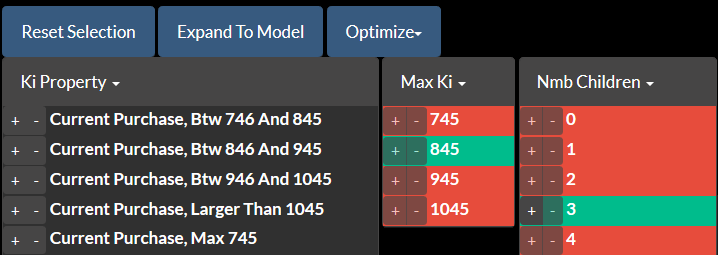
\includegraphics[angle=0,width = 0.6\linewidth]{img/oldscreen_joost.png} %, trim={2.5cm 21,7cm 2,2cm 2,0cm}, clip]
	\caption{Propagation in the original prototype.}
	\label{fig:old}
\end{figure*}
\end{comment}

At the start of the case study the notary's application requirements were rather vague.
The most important concern was to use the obtained information in an intelligent way, i.e., use the information instantly to derive conclusions.
Because of this we opted for the use of the earlier developed \textit{automatic configuration} interface that is available on the \idp homepage \cite{idphome}.
As the use of it is independent of the domain described in the vocabulary and theory in the knowledge base, this was an easy way to create a first visual prototype to solicit further application requirements from the notary.
%Figure \ref{fig:old} shows a screenshot of the original prototype that was developed in \cite{ruleml/DeryckHVV18} using the technology from \cite{ruleml/DassevilleJJVD16}. The interface allows to construct a partial interpretation: the ``$+$'' serves to assign a unique value to a constant, while the ``$-$'' removes the corresponding value from the domain of the constant.
%Applying propagation then leads to a more precise interpretation $\ci^{prop}$. 
For each propagated atom the corresponding box is colored green if the atom is true in $\ci^{prop}$, and red if it is false. In addition, the user may also invoke model expansion to complete the current partial interpretation into some total model, and optimization to complete it into the model expansion that minimizes the duties that need to be paid. 
%The notary office found the propagation and optimization inferences quite useful but did not see much use for model expansion.

%provides a user the possibility to construct an implicit structure by assigning truth values to all atoms over the modelled vocabulary by clicking $+$ (meaning: true) or $-$(meaning: false).
%As a result, the atom is highlighted in green resp. red.

%The development and characteristics of the original interactive decision enactment system (\ides) were described in \cite{Ingmar}, and its application in the registration duty domain in \cite{ruleml/DeryckHVV18}.
\begin{comment}

At the start of the case study the notary's application requirements were rather vague.
The most important concern was to use the obtained information in an intelligent way, i.e., use the information instantly to derive conclusions.
Because of this we opted for the use of the earlier developed \textit{automatic configuration} interface that is available on the \idp homepage \cite{idphome}.
As the use of the \ides~is independent of the domain described in the vocabulary and theory in the knowledge base, this was an easy way to create a first visual prototype to solicit further application requirements from the notary.
\end{comment}
%The interface provides a user the possibility to construct an implicit structure by assigning truth values to all atoms over the modelled vocabulary by clicking $+$ (meaning: true) or $-$(meaning: false).
%As a result, the atom is highlighted in green resp. red.
%Figure \ref{fig:old} shows a screenshot of this interface.



%The inferences performed by the original \ides are propagation, optimization and model expansion.

%\paragraph{Propagation}
%After the user has chosen some atoms' truth values, the consequences of these choices are automatically calculated by \idp's propagation inference. 
%The output of this inference is a set of atoms that hold in all models to the current set of choices. The resulting true atoms are highlighted in green, the false ones in red.
%This allows the user to see the impact of his selections at a glance.
%For experienced users, this is helpful in determining which other parts of information should be requested.
%\jo{last sentence needed?}

%In Figure \ref{fig:old}, the number of children is chosen to be three by assigning the corresponding atom to true, and from this follows that the maximum \textit{kadastral income} (KI) is 845.
%Both are highlighted in green, while the red atoms represent now impossible choices.

%\paragraph{Optimization}
%In complex situations, multiple combinations of \textit{abattement} and registration type might be possible, each leading to an other duty to be paid.
%Typically buyers would prefer to use the option that minimizes this amount, which is calculated by using the optimization inference in the interface.
%For this functionality, we added the following objective function:
%\[
%(BaseAmount * ApplicableRate)- TotalPortability
%\]

%\paragraph{Model expansion}
%The expansion of an incomplete structure to a model that satisfies the theory can be useful for training or validation purposes.
%E.g., if the notary wants to explain to a client in which cases he would be entitled to the rate for social dwellings, he might do this by enforcing the atom assignment $HasRegistrationType=socialDwelling \mapsto \true$ and generating a model.
%\jo{is dit het juiste atoom? Ik ben niet meer zeker van m'n aanpassing...}

\section{Law amendments and the KBP}
\label{law}

%As suggested by \cite{Bench-Capon1992} we started the formalization of the domain with the creation of an intermediate representation of the domain.
As the former version of the legislation concerning registration duties  was unstructured and difficult to read, the model was built on more accessible information from the Federal Public Service Finance \cite{FODFinancien}. 
We analyzed and formalized the domain using the Decision Model and Notation (DMN) methodology.\footnote{The reasons and way of working with DMN are discussed in our earlier work, see \cite{ruleml/DeryckHVV18}.}
This resulted in a model consisting of a glossary and multiple connected decision tables. 
This was then translated into the IDP-language.
The result is an initial prototype that formalizes 11 articles of law, resulting in a knowledge base of 53 concepts, 6 constraints and 14 rules \cite{ruleml/DeryckHVV18}. Building this knowledge base required an effort of approximately 10 person-days.
A significant part of this time was attributed to the creation of the set of symbols representing concepts in the domain (i.e. the \emph{vocabulary}. %In this phase some design choices need to be made, e.g., use of \emph{reification} for auxiliary concepts, or the choice between the use of a function or a relation.  
To this end some analysis beyond the level of the DMN model was needed.

To evaluate the maintainability of the knowledge base, we examined the effort necessary to update it to the changes in legislation enacted in 2018. 
These changes consisted of 5 new articles, making it the most significant change to real estate sales law since the transfer of jurisdiction from the national to the Flemish regional government in 2013. %\footnote{The decree of July 17 2015 made small amendments to a larger number of articles, but only introduced 3 new articles.} 
At the time of constructing the original knowledge base, the content of these changes was not yet known.
Therefore, this provides a realistic test case to judge the maintainability of the knowledge base.

Updating the knowledge base required only $0.5$ person-days, a fraction of the time required for the initial version. 
16 of the original 53 concepts were removed and 18 new ones added; 11 existing constraints and rules needed to be updated or deleted, while 4 new constraints were added. 
Crucially, 9 of the 20 existing constraints/rules did not need to be touched at all. 
This demonstrates that the inherent modularity of the KBP indeed leads to significant advantages in practice.

\begin{comment}


To give an idea of the required changes, we briefly discuss an example.

%that were required to the knowledge base, we briefly provide some examples.
%The dependency between the \textit{kadastral income} and the number of children as demonstrated in figure \ref{fig:old} is formalized in the definition below.
%As the concept of \textit{kadastal income }is eliminated in the new law, this piece of code is deleted in the new program.
%\begin{align*}
%\{ & MaxKi = 745 \leftarrow 0 \leq NmbChildren \leq 2. \\
%& MaxKi = 845 \leftarrow 3 \leq NmbChildren \leq 4.\\
%& MaxKi = 945 \leftarrow 5 \leq NmbChildren \leq 6.\\
%& MaxKi = 1045 \leftarrow 7 \leq NmbChildren. \}
%\end{align*}
In the original prototype, the $RegistrationType$ is defined by a number of rules such as:
%Determination of the registration type is modelled as a definition with multiple rules in which the defining rules from the different types are described. 
%For the legislation prior to June 2018, the structure of the definition was the following (the formulas representing the effective conditions are abstracted and represented by \textit{conditionsOld} resp. \textit{conditionsNew}):
\[\left\{\begin{aligned}
 RegistrationType = Social &\leftarrow \varphi_1.\\
 RegistrationType = Modest &\leftarrow \varphi_2.\\
& \cdots
\end{aligned}\right\}\]
%& HasRegistrationType = commercialPurchase \leftarrow conditionsOld.\\
%& HasRegistrationType = other \leftarrow HasRegistrationType \neq socialDwelling \\
%& \indent \wedge HasRegistrationType \neq modestDwelling\\
%& \indent \wedge HasRegistrationType \neq commercialPurchase. \}
%\end{align*}
After the amendments, new registration types needed to be added (e.g., $Monument$), while some disappeared (e.g., $Modest$) and others remained unchanged (e.g., $Social$).
Thanks to the modular nature of rule-based definitions, these correspond to local changes that preserve the global structure of the definition:
\[\left\{\begin{aligned}
 RegistrationType = Social &\leftarrow \varphi_1.\\
 RegistrationType = Monument &\leftarrow \varphi'.\\
& \cdots
\end{aligned}\right\}\]
%\begin{align*}
%\{ & RegistrationType = socialDwelling \leftarrow conditionsOld.\\
%& HasRegistrationType = familyDwelling \leftarrow conditionsNew.\\
%& HasRegistrationType = withEnergyRenovation \leftarrow %conditionsNew.\\
%& HasRegistrationType = monument \leftarrow conditionsNew.\\
%& HasRegistrationType = commercialPurchase \leftarrow conditionsOld.\\
%& HasRegistrationType = other \leftarrow HasRegistrationType \neq socialDwelling \\
%& \indent \wedge HasRegistrationType \neq familyDwelling\\
%& \indent \wedge HasRegistrationType \neq withEnergyRenovation\\
%& \indent \wedge HasRegistrationType \neq monument\\
%& \indent \wedge HasRegistrationType \neq commercialPurchase. \}
%\end{align*}
%\jo{Hebben we effectief de accolades rond de rules nodig?}
%\Marjolein{naar analogie met de voorbeelden in sectie 3 zou ik dit wel doen}
%The initial analysis of the domain took a considerable amount of time, as the modeller did not have any prior domain knowledge.
%Note that, especially with the approach used, the prior analysis of the domain and its formalization with the use of DMN could be done by a domain expert \cite{iets over DMN en gebruik door business users}.
%However, some additional analysis and understanding of the domain by the \idp-modeller is needed, as certain formulation choices impact the way variables are presented by the interface \cite{Marjolein}.

%Typical for the former regulation was the use of multiple versions of the same concept at different law articles.
%E.g., the definition of 'first property' and the establishment obligation were interpreted differently in the context of the type of real estate (TRE) and the context of abattement.
%\begin{sidewaysfigure}
%\begin{figure}[h]
%    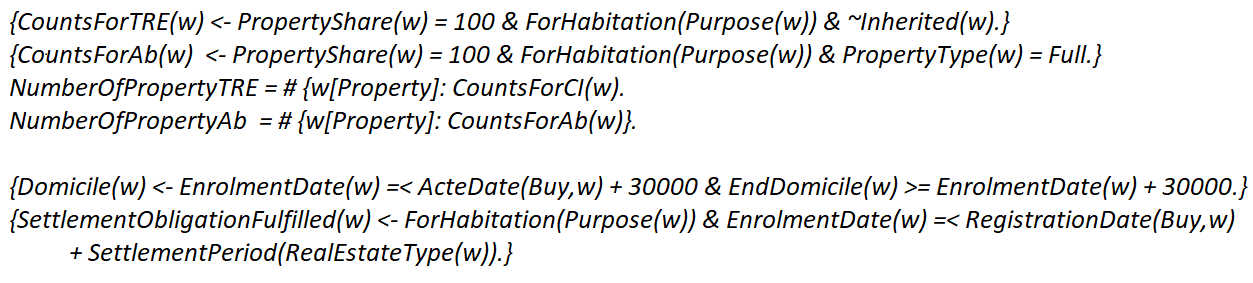
\includegraphics[angle=0,width = 1\linewidth]{img/codeOld.png}
  	%\caption{geen captation:voorbeeldcode.}
%	\label{fig:code}
%\end{figure}
%\end{sidewaysfigure}
%\jo{What is the purpose of this code?}

%\subsubsection{Regulation as from June 1st 2018}
%As discussed above, the regulation changed considerably as from June 1st 2018.
%In our application we modelled the new regulation (without transitional measures for transactions concluded prior to June 1st but registered after this date).
%One of the claims of KBP is that it allows agile adaptations, as all and only conditions are centralized in the concise knowledge base.
%It took a half day of work to implement the profound changes that were described in \ref{sec:background}: two hours were needed to search, analyze and model the new legislation using DMN; and an additional hour and a half were needed to amend the IDP-code. %exacte timings opzoeken%

\end{comment}
 \section{Improved prototype}
\label{interface}

The new interface contains usability updates, such as information tooltips, custom input fields and a start screen with a limited set of predetermined \emph{core} constants.
%hover-over tooltips to explain the meaning of the constants and custom input fields for numerical domains. The user is also initially presented with a small set of predetermined \emph{core} constants, and can expand this set to \emph{relevant} constants 
%\footnote{See further in Section~\ref{interface} for more information on relevance.}
%or simply \emph{all} constants.
%: initially, only constants with the highest priority are shown and the user must expand the view to see also constants of a lower priority. 
A more important improvement is the clear distinction between  \emph{chosen atoms} (set by the user) and  \emph{propagated atoms} (implied by the chosen atoms).
The interface visualizes chosen atoms by a $\circlearrowleft$-symbol to indicate that this choice can be reconsidered. Propagated atoms are visualized by question marks, indicating that they can be \emph{explained}.
%\paragraph{First interactive decision enactment interface}
%In legislation the use of a large number of concepts that are defined at a very fine-grained level are common.
%Often, the definition themselves contain concepts that need to be defined.
%From an end-user point of view this creates a challenge to keep the interface clear.
%The interface proposed in \cite{Ingmar} does not make a distinction between important, often used concepts and less used concepts.
%All of the available concepts are shown in one screen, which is a disadvantage given the large number of fine-grained concepts.
\begin{comment}
As before, the interface operates independently of the domain knowledge gathered in the knowledge base.
This is still the case in the new interface.
Additionally, a separate \emph{comma separated value} file -- denoted as \emph{the CSV} -- is required as input.
The CSV contains some configuration options and meta-information on the symbols to be used by the \ides.
A first piece of meta-information is a priority value for symbols and atoms. This priority value determines which concepts are shown first to a user.
%Initially, only atoms with priority code $1$ are displayed, while atoms with priority code $2$ are displayed when the view is expanded.
Other pieces of meta-information are information strings for symbols and atoms, which allow the \ides~to elaborate on the intended meaning of symbols and atoms in the knowledge domain.
In this application we used it to reference the applicable law article.
\end{comment}
%Also, these information strings are convenient for explaining concepts that are used in the knowledge domain, but are not really part of it.
%E.g., special rates exist for the purchase of monuments (subject to conditions).
%In our current model, we expect the user to know whether or not the real estate can be classified as a monument, so we treat this as a simple Boolean input.
%However, the criteria for buildings to be monuments are determined in a separate decree, and an information string can refer to this decree.
%To avoid confusion and enable use for less versed users, these fine-grained definitions needed to be modelled in the previous interface, leading to excess literals and code.
%In the new interface, more abstract definitions with textual explanation suffice.
%The user can request these strings by hovering over or clicking on a dedicated information button
%The result is a more focused and concise domain knowledge base.
%Further improvements to the \ides~ comes from the new inferences of \textit{relevance} and \textit{explanation}, that are discussed in the following sections.
The most significant improvement is the application of the  \textit{relevance} and \textit{explanation} inferences for interactive decision enactment. 
%Both are refinements of algorithms that already existed in \idp, but that had not yet been used in the context of interactive decision enactment. 

\paragraph{Explanation} to increase user confidence, it is important that the system is able to explain why it derived certain conclusions. 
%At times the use of the \ides~ may lead to unanticipated or even unwanted outcomes, where a user did not expect a propagated atom to be set to true or false.
Moreover, the user sometimes would like to flip a propagated atom's truth assignment.
%In this situation, it is crucial that the propagated atom assignments are explained to clients.
%The identification of chosen atom assignments allows the user to revise his choices and perhaps change the outcome of his query.
%
The explanation inference identifies the chosen atoms that imply a propagated atom, and allows to revise these choices.
%\jo{I refined the inference, but at its core, the inference was already implemented in \idp. Should we mention any of this?}
%\Marjolein{we already mention something similar for the relevance inference. maybe we extend the remark to explanation, rather than repeating it here? --- hm, ik dacht dat dit ergens algemeen vermeld was, maar ik zie  nu dat het bij relevance staat. dan kan je het moeilijk algemener maken natuurlijk.  Als er al over gepubliceerd is, kan je er best ook naar verwijzen, niet?}
As input, it takes a theory $T$, a partial interpretation $\ci$ and a propagated atom $a$. %Propagated assignments (i.e., those that were not chosen by the user but derived by the \emph{propagation} inference) are 
%a shared vocabulary, as well as a single atom assignment $a \mapsto v$ (with $v \in \{\true,\false\}$) propagated from $T$ and $I$.
%More formally, $I \cup \{a \mapsto \neg v\} \not \models T$, or $I$ extended with $a \mapsto \neg v$ can not be expanded to a model for $T$.
As output, it returns a least precise partial interpretation $\ci^{expl}$ such that $a$ would still be propagated by $\ci^{expl}$.
%minimal set of atom assignments $A$ from $I$ such that for structure $I'$ formed by merging $A$ with $I$'s type interpretations, it holds that $I' \cup \{a \mapsto \neg v\} \not \models T$.
%In words, the explanation inference calculates a minimal substructure $I'$ of $I$ that still propagates $a \mapsto v$ under $T$.
\begin{figure}[]
	%\centering	
	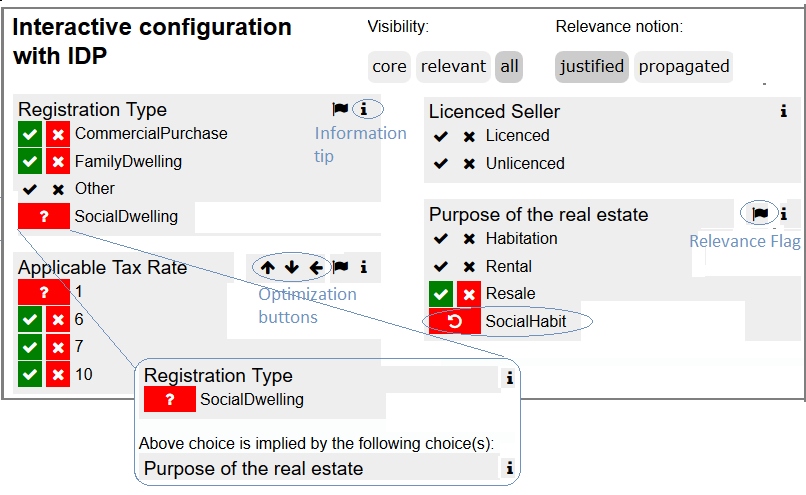
\includegraphics[angle=0,width = 1 \columnwidth]{img/26102018quat.png} %, trim={2.5cm 21,7cm 2,2cm 2,0cm}, clip]
	\caption{Relevance and explanation demonstrated in the new interface.}
	\label{fig:relevance}
\end{figure}
This is demonstrated in Figure~\ref{fig:relevance}.
When a user clicks on the question mark of a propagated atom $a$, the system constructs the partial interpretation $\ci_{chosen}$ from all the chosen atoms, and feeds $a$ and $\ci_{chosen}$ to \idp's explanation inference together with the theory $T$ containing all domain knowledge. The output then represents a minimal subset of all chosen atoms that still imply $a$'s propagated value, which is presented to the user as an explanation for the propagation.
%An overlay pops up, summarizing the minimal set of user choice atoms leading to the propagated atom.
%As shown in Figure~\ref{fig:relevance}, the user can consult the related law article directly by using the information button in the explanation box.

\begin{comment}
\Marjolein{Figure \ref{fig:interface} shows an edited screenshot of this process. The user has requestfed an explanation for the atom $RegistrationType=familyDwelling \mapsto \true$.
The overlay contains the user inputted atoms $TypeOfPurchase=naturalPerson \mapsto true$ and $PurchasePrice=210$, but does not include the user choice of $TypeOfPurchaser=naturalPerson \mapsto \true$, which is not part of an explanation for $RegistrationType=familyDwelling \mapsto \true$.}
\Marjolein{te vervangen door onderstaand stuk}


%\jo{Todo: figuur toont 2 explanations, tekst vertelt over 1.}
%\Marjolein{zal eerst je tekst een nalezen dan :-)}

\begin{example}
\label{ex:explanation}
Starting from example \ref{ex:voctheostruct} we extend theory $T_{ex}$ in which the ApplicableRate is defined with the following definitions of registration type, the allowed selling price limit for family dwellings and a trivial constraint:
\begin{align*}
&\{ HasRegistrationType = socialDwelling \leftarrow Seller = licensedSeller \\
& \indent \wedge Purpose = socialHabitation. \\
& HasRegistrationType = familyDwelling \leftarrow BuyerType = naturalPerson \\
& \indent \wedge Price \leq Limit. \\
& HasRegistrationType = other \leftarrow HasRegistrationType \neq socialDwelling \\
& \indent \wedge HasRegistrationType \neq familyDwelling.\} \\
& \exists x \colon HasRegistrationType = x.\\
&\{Limit = 220 <- Municipality = Antwerp \vee Municipality = Brussels.\\
&Limit = 200 <- Municipality = otherMunicipality.\}
\end{align*}
Input structure $I_{ex}$ is expanded with:
 \begin{align*}
 & BuyerType^I = \{naturalPerson\}\\
 & Price^I = \{220\}\\
 & Municipality^I = \{Antwerp\}
 \end{align*}

% results in the following atoms after propagation
%As the result of the propagation of structure $I_{ex}$ over $T_{ex}$  $a \mapsto v$ with $v\in \{\true\}$:
The propagation of structure $I_{ex}$ over $T_{ex}$ rsults in the following atoms:
 \begin{align*}
     atoms^I = \{
& HasRegistrationType=familyDwelling \mapsto \true, \\
& ApplicableRate=7 \mapsto \true, \\
& BuyerType=naturalPerson \mapsto \true,\\
& Municipality=Antwerp \mapsto \true,\\
& Price=210 \mapsto \true,\\
& Limit=220 \mapsto \true,\\
& HasRegistrationType=other \mapsto \false,\\
& HasRegistrationType=socialDwelling \mapsto \false,\\
& ApplicableRate=1 \mapsto \false,\\
& ApplicableRate=10 \mapsto \false,\\
& Limit=200 \mapsto \false \}
\end{align*}
If the user requests an explanation for the atom ApplicableRate=7 $\mapsto \true$, the inference \textit{explanation} searches for the minimal set of atoms in $I_{in}$ that explain the interpretations in $I_{out}$.  For this example the $ApplicableRate$ is determined by the $BuyerType$, $Municipality$ and $Price$, as shown in figure \ref{fig:interface}.
\end{example}
\begin{figure}[h]
	\centering	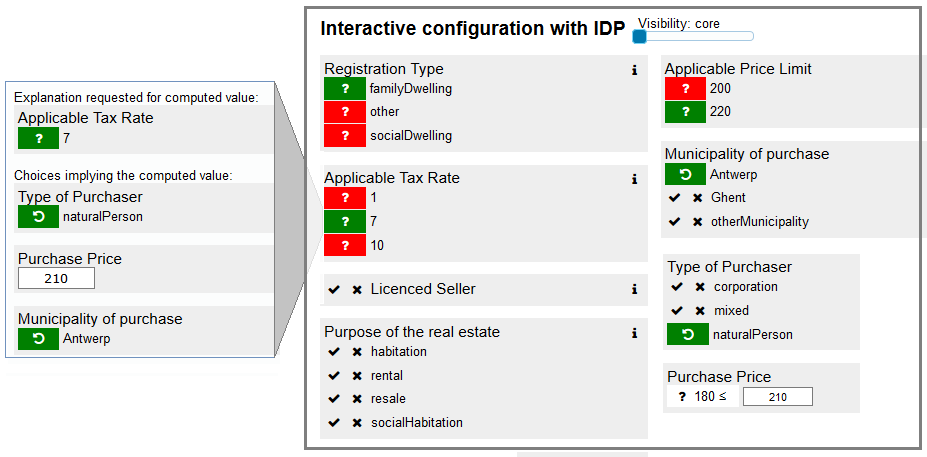
\includegraphics[angle=0,width = 1
	\linewidth]{img/explanation.png} %, trim={2.5cm 21,7cm 2,2cm 2,0cm}, clip]
	\caption{Propagation and explanation in the new \ides.}
	\label{fig:interface}
\end{figure}
\end{comment}
 
\paragraph{Relevance}
\label{sec:relevance}
A key problem of the original prototype was that it encouraged notaries to ask irrelevant questions. For instance, the knowledge base included the concept of a \emph{licensed seller}: only when the seller is licensed, can the property be eligible for a social registration. In particular, the definition of $RegistrationType$ contains the following rule:
\[\left\{\begin{aligned}
 & RegistrationType = Social \leftarrow \\ 
 & Seller=Licensed~\land~Purpose=SocialHabit.
\end{aligned}\right\}\]
Moreover, this is the only formula where the licensed seller concept is used. Once the notary has determined that the purpose of the real estate is not social habitation, there is no longer any need to determine whether the seller is licensed. %However, the original prototype would keep on displaying this as an undecided atom, tempting the notary into inquiring about it.

%In Section \ref{original}, some of the difficulties and solutions to design a clear interface given the inherent complexity of legislation, were discussed.
%In this section we discuss the \emph{relevance} inference as an important aid to keep track of necessary parts of information.
%Also, the relevance inference allows the system to signal the user that a current configuration of incomplete atom assignments suffices to satisfy all constraints in the problem domain, avoiding choices on irrelevant atoms.

%Informally, relevance inference pinpoints all unassigned atoms that can still contribute to satisfying a not yet satisfied constraint. Conversely, all unassigned atoms that have no possible impact on the truth value of any constraint are considered irrelevant.

Our new prototype makes use of the relevance inference to avoid this problem. This inference takes as input a theory $T$, a partial interpretation $\ci$ that is closed under propagation, and a set of \emph{goal constants} $C$. 
Its output is a set of \emph{relevant} atoms $a=v$ that can still affect the interpretation of the constants in $C$, given $T$ and the information present in $\ci$. 
In our example, if $\ci$ is such that $SocialHabit \in Purpose^\ci$ and $C = \{RegistrationType\}$, then the atom $Seller = Licensed$ is relevant, as choosing its truth value determines whether $RegistrationType=Social$.
If $SocialHabit \not\in Purpose^\ci$, then $RegistrationType=Social$ is false in all model expansions of $\ci$ w.r.t.~$T$, and $Seller = Licensed$ is therefore not relevant.
%The constants in $C$ will be called the \emph{goal constants}.

\idp's relevance inference is 
%a refinement of methods that were initially developed in order to improve \idp{}'s internal search routines~\cite{ijcai/JansenBDJD16}. %, but the registration duty use case motivated the development of a full-fledged relevance inference.
%The notion of relevance 
%It is 
based on justification theory (e.g., \cite{lpnmr/DeneckerBS15}). 
% As mentioned in Section~\ref{KBP}, the language that we use in this paper is a highly simplified version of the real \fodot language used in \idp. 
The concepts we introduce in the following paragraphs are highly simplified versions of the original justification theory and of the implementation of the relevance inference that is available in our software tool. %, of which we describe a simplified version here.

%\jo{The following is too detailed for a 4-page paper. I would prefer a reference to Joachim's relevance paper instead.}
The \emph{dependency graph} of a theory $T$ has all of the subformulas of the theory as its nodes and has an edge from each formula to all of its subformulas. In addition, for each rule of the form $A \leftarrow \varphi$, there is also an edge from the atom $A$ to the formula $\varphi$. Intuitively, each directed edge from $\varphi$ to $\psi$ in this graph means that the truth of $\varphi$ is defined (or can be \emph{justified}) by the truth of $\varphi$. Finally, we also add each of the goal constants $C$ to the graph and include an edge from each goal constant $c \in C$ to all atoms of the form $c=v$. The idea behind these edges is that value of the goal constant $c$ is influenced by the truth of these atoms $c=v$. We denote the resulting graph by $G^C_T$.
\begin{comment}
Figure \ref{fig:dependency} demonstrates the dependency graph for our limited example in which the applicable rate is determined by the registration type.



\begin{figure*}[]
	\centering	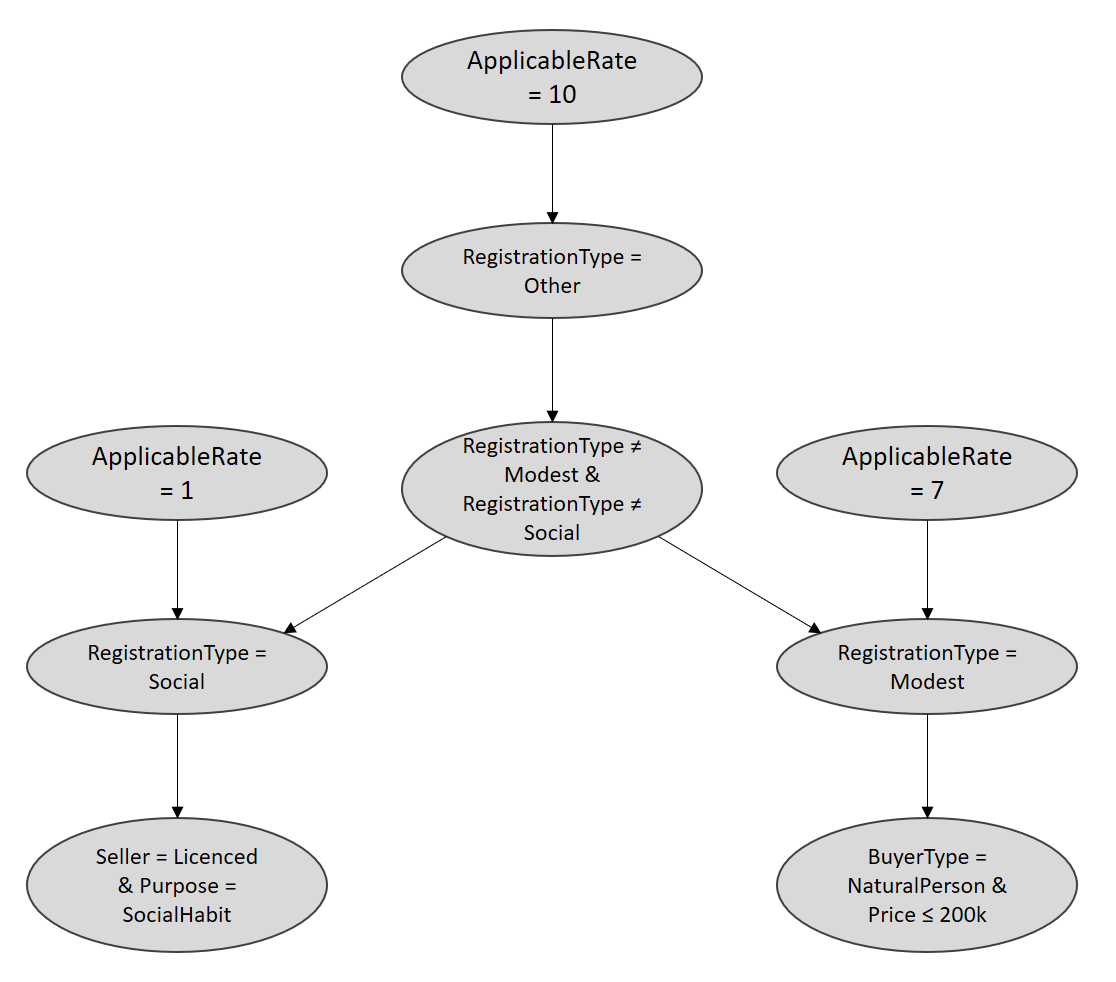
\includegraphics[angle=0,width = 0.6
	\linewidth]{img/dependency.png} %, trim={2.5cm 21,7cm 2,2cm 2,0cm}, clip]
	\caption{Dependency graph for the example theory.}
	\label{fig:dependency}
\end{figure*}
\end{comment}
%The sinks of $G^C_T$ are all atoms that do not appear in the head (i.e., at the left of the $\leftarrow$ symbol) of any rule in $T$. We call these sinks the \emph{open atoms} $Open(G^C_T)$ of the graph; intuitively, their truth value does not depend on that of any other node in the graph. By $\ci\lvert_{Open(G^C_T)}$ we denote the least precise partial interpretation $\ci'$ that such that, for each atom $c=v$ in $Open(G^C_T)$, $c^\ci = c^{\ci'}$. 
We say that a formula $\varphi$ is $T$-\emph{determined} by $\ci$ if either $\ci \models_T \varphi$ or $\ci \models_T \lnot \varphi$. Finally, we define that an atom $c=v$ is \emph{relevant} if it is not $T$-determined by $\ci$ and there exists a path in $G^C_T$ from this atom to one of the goal atoms, which does not traverse any node that is $T$-determined by $\ci$. %$\ci\lvert_{Open(G^C_T)}$.
%Intuitively, an atom is relevant if its truth value may affect the value assigned to one of the goal atoms \emph{and} this possible effect is not blocked by the fact that the truth value of some intermediate formula is already fixed by the current partial interpretation. In case of the above example, $Purpose \neq SocialHabit$ would $T$-imply $RegistrationType \neq Social$ and therefore making this choice would make $RegistrationType = Social$ $T$-determined. Hence, $RegistrationType = Social$ blocks the path from $Seller = Licensed$ to the goal constant $RegistrationType$, making this atom irrelevant. 

%This basic notion of relevance can be further refined in order to better handle special cases such as unfounded choices and recursive definitions~\cite{ijcai/JansenBDJD16}, but this is out of scope of this paper.

%To define what relevant atoms are, we need the notion of a \emph{dependency graph} of a theory.
%A theory's dependency graph has a theory's formulas as nodes, and has a directed edge from a formula to its subformulas, or from a formula in the head of a rule to the formula acting as the body of a rule.\jo{citation needed}
%By a process called \emph{grounding} using a structure's type interpretations, the dependency graph can be simplified such that each node is a unique atomic formula -- an atom.
%Atoms that have no outgoing edges in the dependency graph are called \emph{open}, atoms that have no ingoing edges are \emph{root}.
%In the registration duty use case, the dependency graph is acyclic, thus it forms a tree. \jo{is this "tree-ness" needed?}

%\begin{definition}
%Let $G_T$ be a dependency graph of a theory $T$ with only atom nodes, and let $I$ be a structure over $T$'s vocabulary which is closed under propagation with $T$ and which can be expanded to a model for $T$.
%An atom $a$ is \emph{justified} if $a \mapsto v$ with $v \in \{\true,\false\}$ is in $I$, if there exists a substructure $open(I)$ of $I$ where all true or false atoms are open in $G_T$, and where $open(I) \cup \{a \mapsto v\} \not \models T$ for some $v \in \{\true,\false\}$.
%\end{definition}
%Informally, an atom is justified if its truth value is fixed by an assignment to open atoms.

%\begin{definition}
%Let $G_T$ be a dependency graph of a theory $T$ with only atom nodes, and let $I$ be a structure over $T$'s vocabulary which is closed under propagation and which can be expanded to a model for $T$.
%An atom $a$ is \emph{relevant} if it is not justified by $G_T$ and $I$, and if it is reachable in $G_T$ from an unjustified root atom by only traversing unjustified atoms.
%\end{definition}
%Informally, root atoms in a dependency graph represent constraints in $T$, and relevant atoms are those that might still justify an unjustified constraint.

%Now, the relevance inference takes as input a theory $T$ and structure $I$ over a shared vocabulary, such that $I$ is closed under propagation with $T$ and $I$ can still be expanded to a model of $T$, while its output is simply the set of atoms relevant under $T$ and $I$.

%\begin{example}
%\label{ex:relevance}
%\Marjolein{code verplaatst naar explanation : Consider the following theory which defines the registration type and has a trivial constraint:
%\begin{align*}
%\{ & HasRegistrationType = socialDwelling \leftarrow Seller = licensedSeller \\
%& \indent \wedge Purpose = socialHabitation. \\
%& HasRegistrationType = familyDwelling \leftarrow BuyerType = naturalPerson \\
%& \indent \wedge Price \leq Limit. \\
%& HasRegistrationType = other \leftarrow HasRegistrationType \neq socialDwelling \\
%& \indent \wedge HasRegistrationType \neq familyDwelling.\} \\
%& \exists x \colon HasRegistrationType = x.
%\end{align*}

%In case the estate has not been destined for social habitation, we can construct a structure $I$ with only assigned atoms $Purpose = socialHabitation \mapsto \false$ (the estate's purpose can not be social habitation) and the implied $HasRegistrationType=socialDwelling \mapsto false$ (the registration type can not be a social dwelling).}
%Consider the theory from example \ref{ex:explanation} and an  interpretation $I_{rel}$ that contains the assigned value for $Purpose$ and the propagated value for $socialDwelling$:
%\begin{align*}
%    &Purpose = socialHabitation \mapsto \false\\
%    &HasRegistrationType=socialDwelling \mapsto \false
%\end{align*}

%$I$ is closed under propagation with $T$, but there still exists an expansion of $I$ to a model of $T$.
%Now, the output of the relevance inference with $T$ and $I$ as input will not contain the atom $Seller=licensedSeller$, as it could only be reached from the constraint $\exists x \colon HasRegistrationType = x$ through the node $HasRegistrationType = socialDwelling$, which is justified as $Purpose = socialHabitation\mapsto false$ is an open, assigned value in $T$'s dependency graph.
%In other words, whether the seller of the estate is a licensed seller, is not relevant, and it is not needed to fix the value of the corresponding atom.

%Similarly, if the registration type is not a social dwelling or a family dwelling, the registration type must be ``other'', satisfying the unique constraint, and making any further unassigned atoms irrelevant.
%%in praktijk na te kijken of dit ook zo in de interface aangegeven wordt!
% iets toe te voegen over constraint
%\Marjolein{ik zou de laatste zin weglaten: het principe wordt reeds duidelijk uitgelegd voor licencedSeller}
%\end{example}

In the interface, a relevant choice $c=v$ is highlighted with red and green buttons (to assign it true or false), while irrelevant choices can still be made, but the buttons are grey. In addition, the box for a constant $c$ is flagged in the upper right corner to indicate that at least one relevant atom over $c$ still exists. Finally, it is also possible to hide irrelevant unknown atoms. %The choices of the relevant atoms themselves are highlighted in green and red.
Figure \ref{fig:relevance} shows the atom $Seller=Licensed$ is indeed irrelevant (for the implicit goal constant $RegistrationType$) under the given truth assignment.




\section{Related Work}
\label{related}
We are not the first to model legislation into a logic-based language.
In the United Kingdom, several pieces of legislation were represented as executable logic programs \cite{cacm/SergotSKKHC86, icail/Bench-CaponRRS87}.
%For instance, the British Nationality Act  and a large part of the Supplementary Benefit Legislation \cite{icail/Bench-CaponRRS87} were modelled in Prolog.
Later, a shift from logic programs to description logic knowledge bases occurred \cite{valente1995legal, ijmms/KralingenVBH99}. %Early examples include Valente's functional ontologies \cite{valente1995legal} and Van Kralingen's frame-based ontologies \cite{ijmms/KralingenVBH99}.
These are simpler, decidable logics for which the decision procedures are tractable for a machine.
However, this also comes at a cost: by limiting complexity, expressivity is often limited as well. Hence, to express a complex legal statement, auxiliary symbols will often be required.
In the extreme case, it might not even be possible to express certain laws.

Nevertheless, there have been European projects that model legislation into description logic knowledge bases~\cite{HARNESS}.
%, and its successors \cite{AGILE, jurix/ForheczKMS09}.
Alongside them, XML standards were developed to express such description logic knowledge bases~\cite{lncs/BoerWV08, icail/PalmiraniCV09}.
%Examples include the Legal Knowledge Interchange Format (LKIF) \cite{lncs/BoerWV08}, Akoma Ntoso \cite{BarabucciCPPV09}, and the Legal Metadata Interchange Format (LMIF) \cite{icail/PalmiraniCV09}.

All research above is focused on a single kind of reasoning (deductive reasoning or satisfiability checking), whereas our approach is multi-inferential by construction. This multi-inferential nature allows us to perform different reasoning tasks all with the same modeled legislation, which is crucial for an interactive decision enactment system.

Regarding the formalization of the legal domain, some interesting suggestions regarding the use of an intermediate model between the knowledge domain and the final knowledge base have been done by \cite{Bench-Capon1992} and \cite{ijmms/KralingenVBH99}.
\begin{comment}
The purpose of this intermediate model is to ensure a thorough analysis of the domain, independent of the implementation goal.
Although we share this concern, we see an additional role for the intermediate model, i.e., to facilitate communication between the domain expert and the modeller.
Therefore we prefer to use the DMN-based tool OpenRules.




The use of the DMN-based tool of OpenRules, allows to define concepts and attributes in a business glossary, while rules are formalized in decision tables.
These parts are analog to the \textit{class hierarchy} and \textit{rule base} parts suggested by \cite{Bench-Capon1992}.
Especially in \cite{Bench-Capon1992}, the importance of an analog structure of the knowledge base and legislation, what they refer to as \textit{isomorphism}, is stressed.
While our program shows some isomorph characteristics %(build on a single legal source, theory represents only the legal source, structure of the articles is partly reflected in the definition)
, we sometimes deviate from the principle.
For example, subsection 2 contains a number of articles that each describe a separate registration type with its applicable tax rate. 
In the knowledge base of our application, the registration type is defined in one definition (with each rule referring to a separate article).
The tax rate however, is defined in a separate definition (referring to the same articles).
The dogmatic use of isomorphism seems less relevant in the limited scope of our application and with the implemented features of explanation and relevance.
\end{comment}

\section{Discussion and Conclusion}
\label{conclusion}

This paper presents an advanced prototype of an interactive decision enactment system, developed to support notaries during client meetings.
It improves the original prototype of \cite{ruleml/DeryckHVV18} in two ways.  First, the knowledge base was updated to reflect  substantial changes to the regulations. % that came into force on June 1st 2018.
Second, new inferences were integrated to meet additional requirements articulated by the notary.

These results validate two central claims of the Knowledge Base Paradigm.
%The experience with this unique case supports the claim from the knowledge base paradigm that knowledge bases are highly responsive to changes in the domain because they only contain actual domain knowledge and are not clouded by inference methods.
First, the effort to update the knowledge base (0.5 person-days) was very small in comparison to the effort to create the initial knowledge base (10 person-days), especially when taking the size of the legal changes into account. This demonstrates the maintainability of an approach based on the KBP. % (13 of the 42 articles were deleted or modifies, and 5 new articles were added). 
%Even when taking possible learning effects into account, this difference stays impressive.
%Second, the improvements to the user interface demonstrate the feasibility of an approach in which the knowledge base is developed separately from the inference methods that can be applied to it. 
Second, it also shows a first-time integration of the relevance and explanation inferences in an interactive application, and demonstrates their practical utility.  
\begin{comment}
In particular, we have implemented two pieces of functionality that were not originally foreseen when the knowledge base was developed, but that were demanded later by the notary office. We did so by applying two fully generic inferences to the existing knowledge base. 

%The re-use of the automatic configuration interface of \cite{ruleml/DassevilleJJVD16} in the first prototype already concretize the claim that inferences can be developed separately from the problem it is intended to be used for.
%This paper helps to build proof for the claim that knowledge bases can be reused by inferences by integrating for the first time inferences of relevance and explanation in the external interface without any need to amend the formulated domain knowledge.

The \emph{relevance} inference addresses the need for efficient information gathering, as it narrows down the entire set of undecided atoms to those that matter for top-level decisions.
This helps the notary avoid requesting superfluous information from his clients.
Once an atom is propagated by the system, the \emph{explanation} inference allows to explore why this particular outcome is implied.



More generally, the contributions of this paper are validation of the claims that knowledge bases are easy to maintain, even in the face of considerable changes in the domain; and that knowledge bases can be reused for other, unanticipated inference tasks.


It also shows a first-time integration of the relevance and explanation inferences in an interactive application, and demonstrates their practical utility.  
\end{comment}
The resulting interactive decision enactment system is applicable to a wide range of applications.
\begin{comment}


We are already investigating another application, coincidentally also in the legal field, is the creation of a knowledge base that supports decision making given the Belgian legislation on public procurement.
Furthermore, it would be valuable to develop a variant of the explanation inference that not only reports a user's choices that lead to a propagation, but also the constraints and/or rules that trigger the propagation. In the legal domain, this would be useful to argue which laws or legal texts enforce a particular outcome under the current choices. E.g., it could point a jurist to a precedent applicable to the case at hand.
\end{comment}
Future work regarding the developed interactive decision enactment system will focus on the use of the system in other legal domains and the application of new generic inferences.


\bibliographystyle{plain} %{splncs}
{\footnotesize
\bibliography{lib,idp-latex/krrlib}}
\end{document}